% =====================================================================
% Decoupled Document Inference — arXiv preprint scaffold.
%
% Ground rules (paper/RESEARCH_PLAN.md, issue #1):
%   1. Every empirical number is rendered from paper/evidence.json, which pins
%      its raw inputs by full SHA-256; see paper/build.sh.
%   2. Missing generated inputs are surfaced as \todoreport stubs so the
%      document still compiles.
%   3. Framing throughout is a *characterization study*: how much
%      cross-document attention can be removed, and what does removing it
%      buy? (RESEARCH_PLAN §12.)
%
% Compile checked-in artifacts:  ./paper/build.sh
% =====================================================================

\documentclass[10pt]{article}

% --- geometry & layout ------------------------------------------------
\usepackage[letterpaper,margin=.8in]{geometry}
\usepackage{parskip}
\setlength{\columnsep}{.25in}
\setlength{\textfloatsep}{7pt plus 2pt minus 2pt}
\setlength{\floatsep}{6pt plus 2pt minus 2pt}

% --- graphics, colour, links ------------------------------------------
\usepackage{graphicx}
\usepackage{caption}
\usepackage{float}
\captionsetup{font=small,labelfont=bf,skip=8pt}
\usepackage{xcolor}
\usepackage[hidelinks]{hyperref}
\usepackage{tikz}
\usepackage{pgfplots}
\usepgfplotslibrary{groupplots}
\pgfplotsset{compat=1.18}
\definecolor{ddiBlue}{HTML}{1263D6}
\definecolor{ddiGold}{HTML}{F07818}
\definecolor{ddiGreen}{HTML}{008C69}
\definecolor{ddiPurple}{HTML}{773BBD}
\definecolor{ddiRed}{HTML}{D1495B}
\setlength{\emergencystretch}{2em}
\raggedbottom

% --- tables & typography ----------------------------------------------
\usepackage{booktabs}
\usepackage{multirow}
\usepackage{xspace}

% --- math -------------------------------------------------------------
\usepackage{amsmath}
\usepackage{amssymb}

% --- bibliography (author-year) ---------------------------------------
\usepackage[round,authoryear]{natbib}
\bibliographystyle{plainnat}

% =====================================================================
% Placeholder helpers.
%
% \todoreport{human message}{regeneration hint}
%   Rendered in place of any table / figure the store cannot yet
%   populate. Sections call this macro when a checked-in artifact is absent so
%   the compiled PDF advertises exactly which sweep unblocks each cell.
% =====================================================================
\newcommand{\todoreport}[2]{%
    \begin{center}%
        \fbox{\parbox{0.9\linewidth}{%
            \textbf{TODO:} #1 --- run \texttt{#2} and re-render.%
        }}%
    \end{center}%
}

% \todo{text} — inline prose stub used by the section audit
% (paper/AUDIT_NOTES.md) to flag claims that need evidence from a future
% experimental pass. Renders as a highlighted bracketed note so a reader
% cannot miss it. Distinct from \todoreport, which stands in for a
% missing table or figure.
\newcommand{\todo}[1]{%
    \textbf{\color{red}[TODO: #1]}%
}

% \figureifexists{path}{caption}{label} — include a generated figure if
% build.sh actually produced it; otherwise fall back to a \todoreport
% stub. Keeps the paper compilable in a container with an empty store.
\newcommand{\figureifexists}[3]{%
    \IfFileExists{#1}{%
        \begin{figure}[t]%
            \centering%
            \includegraphics[width=\linewidth]{#1}%
            \caption{#2}%
            \label{#3}%
        \end{figure}%
    }{%
        \todoreport{figure \texttt{#1} missing}{./paper/build.sh}%
    }%
}

% =====================================================================
% Title block.
%
% Author metadata is approved for this preprint.
% =====================================================================
\title{Prefill Once, Reuse Anywhere?\\
       Quality, Sparsity, and Document KV Reuse in RAG}

\author{Aleksandr Kaigorodov\\
        Yandex\\
        \texttt{alexkay28@yandex-team.ru}}

\date{\today}

\begin{document}

\maketitle

\begin{abstract}
Retrieval-augmented generation (RAG) repeats document prefill across requests.
Decoupled Document Inference (DDI) isolates document attention via a
block-diagonal mask and uses restart positions to make independently computed
document KVs reusable. Block-Attention~\citep{ma2025blockattention} achieves
98.7\% TTFT reduction with full-model fine-tuning; this paper asks how far
lightweight self-distillation goes and what serving boundary remains.
Two approaches compose: \textbf{sparse cold prefill} reduces attention work on
cache misses; \textbf{warm KV reuse} loads stored document states and skips
document prefill. At $N=25,L=512,Q=64$, DDI-QF removes
95.04\% of causal prefill pairs, but measured dense-SDPA prefill remains near the
full-causal latency (the 4D additive mask forces SDPA's slow math backend).
Historical Flex logs report 1.77$\times$ whole-model prefill gain; their older
mask semantics and failed parity gates prevent treating these as validated
current-DDI speedups. Natural-QA mask and document-count studies show quality
losses (HotpotQA EM 0.56$\to$0.30 train-free); matched three-seed self-distillation
(top-8 layers) does not reach prescribed parity gates. A trained link-token
contract (V70) then closes the quality gate: on 300 untouched records, cached
versus fresh generation is \textbf{byte-identical} (C$-$B $=0$, CI $[0,0]$),
replicated at a second seed (V72). The trained contract's serving boundary
(V71) keeps the warm-path win: all-hit TTFT up to 5.55$\times$ with zero
identity violations across 240 cells, winning above hit-fraction crossovers
($h\geq 0.7$ at $L=512$, $h\geq 0.8$ at $L=128$). The win is scoped:
mixed-hit traffic remains slower, and the sparse cold path wins only at long
shapes (1.12--1.29$\times$ at $L=512$). We therefore claim a measured, audited
warm-path speedup with byte-identical serving after contract training --- not
yet a quality-preserving general replacement for full causal attention at scale.
\end{abstract}

% ---------------------------------------------------------------------
% Body — every section is a separate .tex under sections/. Keep the
% split so a section can be reviewed independently from checked-in artifacts.
% ---------------------------------------------------------------------
\section{Two Paths to Less Document Prefill}
\label{sec:thesis}

Retrieval-augmented generation re-encodes the same passages across requests,
but full-causal attention makes their hidden states position-dependent.
Efficient KV memory management \citep{kwon2023pagedattention} does not, by
itself, remove this dependency. DDI changes the attention graph to isolate
documents, then uses restart positions to support independently computed
document states. Two savings are distinguished: a
\textcolor{ddiGold}{\textbf{cold document}} still needs computation confined
to its own block; a \textcolor{ddiGreen}{\textbf{warm document}} can load
previously computed KVs and skip that document's prefill.

\paragraph{Contributions.}
This paper reports a completed validation program with six results:
\begin{enumerate}
\item \textbf{Cache fidelity, exactly.} A canonical execution contract makes
persisted-cache execution coincide with fresh independent execution:
identical document K/V tensors (asserted per record), the same greedy
callable, and exactly equal EM and F1 on all $n{=}300$ confirmation records
(C$-$B $=0$ at every station). This is a property of canonical execution and
persistence correctness, not of link-token training: it holds equally for the
untrained $k{=}0$ arm (seed-1 confirmation) and on Llama-3.1-8B.
\item \textbf{The serving boundary is measured on the same contract.} Against
the untrained-restart monolithic reference (arm A of
Section~\ref{sec:cache}), all-hit TTFT reaches $5.55\times$ and all-hit
wall speedup at decode $d{=}1$ reaches $6.55\times$ ($L{=}512$, $N{=}10$),
across 240 grid configurations at 15 timed repeats each, with zero identity
violations (V71).
\item The 95\%-sparsity $\to$ 0\%-speedup gap under SDPA is an
\textbf{implementation property}, now measured (V101): a 4D additive mask
disables SDPA's flash dispatch and routes the prefill to the
memory-efficient kernel, which reads the full bias and leaves block-sparsity
unexploited ($\sim$1.5$\times$ slower than the 2D path at the 95\%-sparsity
shape; identical for full-causal and 95\%-sparse masks).
\item The trained contract requires its \textbf{mask and layout to cohere}
(V110): executing the trained weights with either pure mode --- the isolated
mask on the contract layout, or a full-causal mask on a plain sequential
stream --- lands near the contract's quality (EM 0.42--0.48), while the
mixed execution inherited from the V70 D arm (full-causal mask on the
restart/link layout) collapses to EM 0.20. Full-causal execution itself is
\emph{not} out-of-distribution for the trained weights.
\item \textbf{A withdrawn baseline, redone genuinely (V112).} Our first
prefix-cache harness had a nonfunctional hit branch and was withdrawn with
root cause; the rebuilt cache stores real document-prefix K/V tensors and
loads them on hits (instrumented: hits forward only query tokens). It wins
fixed-order traffic ($12.2\times$ prefill, $8.5\times$ TTFT) and degrades
exactly to monolithic under document reordering, while DDI's
content-addressed cache keeps its win under both --- at the cost of exact
identity: prefix hits reproduce monolithic outputs on 90\% of requests, not
100\%.
\item All displayed figure values are \textbf{rendered from the sha-pinned
ledger} (including V14--V18), the renderer rejects changed artifacts and
plotted numbers, failed gates stay visible, and a retracted experiment is
documented in-text.
\end{enumerate}

\paragraph{The 2025--2026 landscape.}
Block-Attention~\citep{ma2025blockattention} divides passages into blocks
with independent KV states and \emph{fine-tunes the full model}, reporting a
98.7\% TTFT reduction that combines custom block-sparse prefill kernels with
\emph{precomputed and reused} document KVs. It therefore does not isolate
what a sparse cold-prefill kernel alone achieves, and its quality evaluation
is not a persisted-versus-fresh identity comparison. Our work differs in
training scope (top-8-layer self-distillation), in the fidelity estimand
(exact persisted-vs-fresh execution identity), and in measuring the serving
boundary of the same contract that passes the fidelity gate
(Table~\ref{tab:comparators}).
KVLink~\citep{yang2025kvlink} is the closest method on the caching side: it
caches independent per-document KVs, adjusts positions, inserts a small
number of link tokens (including $K{=}5$) and fine-tunes --- but targets
\emph{quality recovery} after approximate cache reuse, reporting
near-recovery rather than exact execution identity. Sparse
RAG~\citep{zhu2025sparserag} encodes documents in parallel and
selectively attends via control tokens; our approach removes cross-document
attention structurally. LazyAttention~\citep{xia2026lazyattention} solves
the positional-encoding problem by deferring rotation inside attention
kernels; our restart layout targets the same goal via per-document position
restart. ProphetKV~\citep{wang2026prophetkv} uses query-driven token
prioritization to retain 96--101\% of full-prefill accuracy at 20\%
recomputation; our contract achieves exact cached-vs-fresh execution
identity but with $5N$ link-token overhead rather than recomputation. Other
related work --- Writing in the Margins~\citep{russak2024wim},
PCED~\citep{corallo2026pced}, Graph-KV~\citep{wang2025graphkv} --- is
complementary or addresses different inputs.

\begin{table}[H]
\centering\footnotesize
\begin{tabular}{p{0.30\linewidth}p{0.30\linewidth}p{0.30\linewidth}}
\toprule
& KVLink~\citep{yang2025kvlink} / Block-Attention~\citep{ma2025blockattention} & This work \\
\midrule
Document KV handling &
independent per-document caches; Block-Attention precomputes/reuses block KVs &
independent per-document canonical caches with content-addressed identity \\
\addlinespace[2pt]
Positional scheme &
positional adjustment (KVLink); block-local encoding (Block-Attention) &
restart positions per document \\
\addlinespace[2pt]
Link tokens &
yes, $K$ up to 5, learned (KVLink) &
yes, $K{=}5$, \emph{fixed deterministic} marker embeddings \\
\addlinespace[2pt]
Training scope &
fine-tuning (KVLink: full model; Block-Attention: full model) &
top-8-layer self-distillation only \\
\addlinespace[2pt]
Quality estimand &
quality recovery after cache reuse (approximate) &
persisted vs.\ fresh execution identity (exact, gated) \\
\addlinespace[2pt]
Serving characterization &
TTFT reduction with reuse (Block-Attention) &
per-shape serving boundary, TTFT and wall, same contract \\
\bottomrule
\end{tabular}
\caption{Method comparison against the two closest prior systems. Estimands
differ: KVLink reports recovery after approximate reuse; Block-Attention
reports TTFT with precomputed/reused blocks; neither measures exact
persisted-vs-fresh identity.}
\label{tab:comparators}
\end{table}

\section{What Isolation Changes}
\label{sec:mechanism}

DDI-QF preserves causal attention within each document and within the query,
removes cross-document attention, and lets every query row see document
keys. Answer rows attend all document columns, the query, and preceding
answers. At one document, the mask returns full causal attention by
convention.

\begin{figure}[H]
\centering\resizebox{.88\linewidth}{!}{% Generated by paper/render.py; aggregates: paper/evidence.json.
% Sources: VIBEQUEUE-53-REPORT.md sha256=7cd9223e128c5d82b61e59575035fe4bb54c9f48c5da721723fd5d214d85195e; results/cache_v53_local_20260907/summary.json sha256=28ae886d9dae851ed090b7ebb0744b33926060d9499c3f16a01221810a0e2189; results/cache_v53_local_20260907/timing.jsonl sha256=055cf47312269ca147c6d4517d26b82aabc910b11fd6ca07f5eba5e3f54153a8; results/cache_v53_local_20260907/validation.jsonl sha256=8597c0b5394b4b17248065ad1ebc386a0a2d864f089f8e65d51d5e293f7b8d4a; ddi/masks.py sha256=2ee804f18a94f4bd709b7629d4962a7c47f732157284c4218f31239956ba7f54
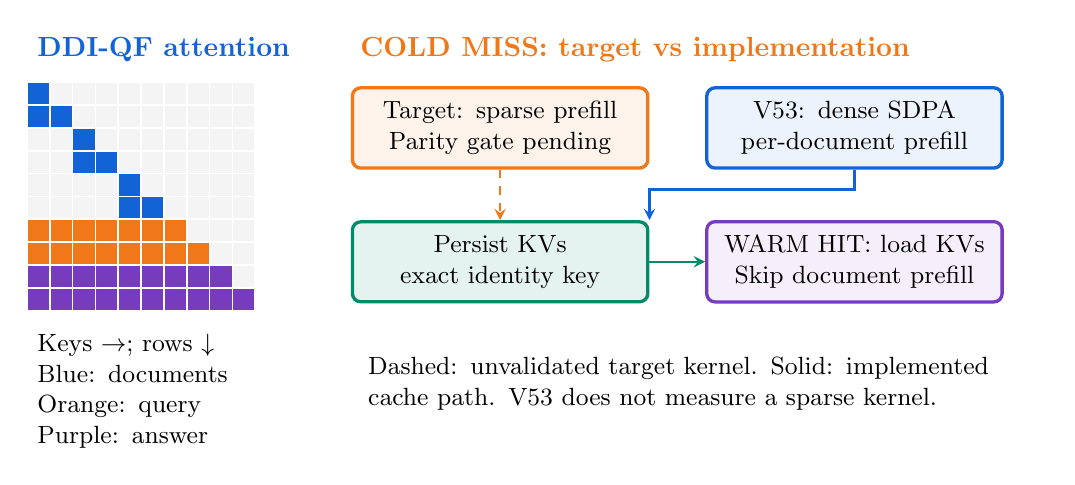
\begin{tikzpicture}[x=1cm,y=1cm,>=stealth,font=\small,box/.style={draw,very thick,rounded corners=3pt,text width=3.4cm,minimum height=1cm,align=center,inner sep=5pt}]
\node[anchor=west,text width=3.5cm,font=\bfseries,text=ddiBlue] at (0,4.3) {DDI-QF attention};
\fill[ddiBlue] (0.00,3.60) rectangle ++(.27,.27);
\fill[gray!9] (0.29,3.60) rectangle ++(.27,.27);
\fill[gray!9] (0.58,3.60) rectangle ++(.27,.27);
\fill[gray!9] (0.87,3.60) rectangle ++(.27,.27);
\fill[gray!9] (1.16,3.60) rectangle ++(.27,.27);
\fill[gray!9] (1.45,3.60) rectangle ++(.27,.27);
\fill[gray!9] (1.74,3.60) rectangle ++(.27,.27);
\fill[gray!9] (2.03,3.60) rectangle ++(.27,.27);
\fill[gray!9] (2.32,3.60) rectangle ++(.27,.27);
\fill[gray!9] (2.61,3.60) rectangle ++(.27,.27);
\fill[ddiBlue] (0.00,3.31) rectangle ++(.27,.27);
\fill[ddiBlue] (0.29,3.31) rectangle ++(.27,.27);
\fill[gray!9] (0.58,3.31) rectangle ++(.27,.27);
\fill[gray!9] (0.87,3.31) rectangle ++(.27,.27);
\fill[gray!9] (1.16,3.31) rectangle ++(.27,.27);
\fill[gray!9] (1.45,3.31) rectangle ++(.27,.27);
\fill[gray!9] (1.74,3.31) rectangle ++(.27,.27);
\fill[gray!9] (2.03,3.31) rectangle ++(.27,.27);
\fill[gray!9] (2.32,3.31) rectangle ++(.27,.27);
\fill[gray!9] (2.61,3.31) rectangle ++(.27,.27);
\fill[gray!9] (0.00,3.02) rectangle ++(.27,.27);
\fill[gray!9] (0.29,3.02) rectangle ++(.27,.27);
\fill[ddiBlue] (0.58,3.02) rectangle ++(.27,.27);
\fill[gray!9] (0.87,3.02) rectangle ++(.27,.27);
\fill[gray!9] (1.16,3.02) rectangle ++(.27,.27);
\fill[gray!9] (1.45,3.02) rectangle ++(.27,.27);
\fill[gray!9] (1.74,3.02) rectangle ++(.27,.27);
\fill[gray!9] (2.03,3.02) rectangle ++(.27,.27);
\fill[gray!9] (2.32,3.02) rectangle ++(.27,.27);
\fill[gray!9] (2.61,3.02) rectangle ++(.27,.27);
\fill[gray!9] (0.00,2.73) rectangle ++(.27,.27);
\fill[gray!9] (0.29,2.73) rectangle ++(.27,.27);
\fill[ddiBlue] (0.58,2.73) rectangle ++(.27,.27);
\fill[ddiBlue] (0.87,2.73) rectangle ++(.27,.27);
\fill[gray!9] (1.16,2.73) rectangle ++(.27,.27);
\fill[gray!9] (1.45,2.73) rectangle ++(.27,.27);
\fill[gray!9] (1.74,2.73) rectangle ++(.27,.27);
\fill[gray!9] (2.03,2.73) rectangle ++(.27,.27);
\fill[gray!9] (2.32,2.73) rectangle ++(.27,.27);
\fill[gray!9] (2.61,2.73) rectangle ++(.27,.27);
\fill[gray!9] (0.00,2.44) rectangle ++(.27,.27);
\fill[gray!9] (0.29,2.44) rectangle ++(.27,.27);
\fill[gray!9] (0.58,2.44) rectangle ++(.27,.27);
\fill[gray!9] (0.87,2.44) rectangle ++(.27,.27);
\fill[ddiBlue] (1.16,2.44) rectangle ++(.27,.27);
\fill[gray!9] (1.45,2.44) rectangle ++(.27,.27);
\fill[gray!9] (1.74,2.44) rectangle ++(.27,.27);
\fill[gray!9] (2.03,2.44) rectangle ++(.27,.27);
\fill[gray!9] (2.32,2.44) rectangle ++(.27,.27);
\fill[gray!9] (2.61,2.44) rectangle ++(.27,.27);
\fill[gray!9] (0.00,2.15) rectangle ++(.27,.27);
\fill[gray!9] (0.29,2.15) rectangle ++(.27,.27);
\fill[gray!9] (0.58,2.15) rectangle ++(.27,.27);
\fill[gray!9] (0.87,2.15) rectangle ++(.27,.27);
\fill[ddiBlue] (1.16,2.15) rectangle ++(.27,.27);
\fill[ddiBlue] (1.45,2.15) rectangle ++(.27,.27);
\fill[gray!9] (1.74,2.15) rectangle ++(.27,.27);
\fill[gray!9] (2.03,2.15) rectangle ++(.27,.27);
\fill[gray!9] (2.32,2.15) rectangle ++(.27,.27);
\fill[gray!9] (2.61,2.15) rectangle ++(.27,.27);
\fill[ddiGold] (0.00,1.86) rectangle ++(.27,.27);
\fill[ddiGold] (0.29,1.86) rectangle ++(.27,.27);
\fill[ddiGold] (0.58,1.86) rectangle ++(.27,.27);
\fill[ddiGold] (0.87,1.86) rectangle ++(.27,.27);
\fill[ddiGold] (1.16,1.86) rectangle ++(.27,.27);
\fill[ddiGold] (1.45,1.86) rectangle ++(.27,.27);
\fill[ddiGold] (1.74,1.86) rectangle ++(.27,.27);
\fill[gray!9] (2.03,1.86) rectangle ++(.27,.27);
\fill[gray!9] (2.32,1.86) rectangle ++(.27,.27);
\fill[gray!9] (2.61,1.86) rectangle ++(.27,.27);
\fill[ddiGold] (0.00,1.57) rectangle ++(.27,.27);
\fill[ddiGold] (0.29,1.57) rectangle ++(.27,.27);
\fill[ddiGold] (0.58,1.57) rectangle ++(.27,.27);
\fill[ddiGold] (0.87,1.57) rectangle ++(.27,.27);
\fill[ddiGold] (1.16,1.57) rectangle ++(.27,.27);
\fill[ddiGold] (1.45,1.57) rectangle ++(.27,.27);
\fill[ddiGold] (1.74,1.57) rectangle ++(.27,.27);
\fill[ddiGold] (2.03,1.57) rectangle ++(.27,.27);
\fill[gray!9] (2.32,1.57) rectangle ++(.27,.27);
\fill[gray!9] (2.61,1.57) rectangle ++(.27,.27);
\fill[ddiPurple] (0.00,1.28) rectangle ++(.27,.27);
\fill[ddiPurple] (0.29,1.28) rectangle ++(.27,.27);
\fill[ddiPurple] (0.58,1.28) rectangle ++(.27,.27);
\fill[ddiPurple] (0.87,1.28) rectangle ++(.27,.27);
\fill[ddiPurple] (1.16,1.28) rectangle ++(.27,.27);
\fill[ddiPurple] (1.45,1.28) rectangle ++(.27,.27);
\fill[ddiPurple] (1.74,1.28) rectangle ++(.27,.27);
\fill[ddiPurple] (2.03,1.28) rectangle ++(.27,.27);
\fill[ddiPurple] (2.32,1.28) rectangle ++(.27,.27);
\fill[gray!9] (2.61,1.28) rectangle ++(.27,.27);
\fill[ddiPurple] (0.00,0.99) rectangle ++(.27,.27);
\fill[ddiPurple] (0.29,0.99) rectangle ++(.27,.27);
\fill[ddiPurple] (0.58,0.99) rectangle ++(.27,.27);
\fill[ddiPurple] (0.87,0.99) rectangle ++(.27,.27);
\fill[ddiPurple] (1.16,0.99) rectangle ++(.27,.27);
\fill[ddiPurple] (1.45,0.99) rectangle ++(.27,.27);
\fill[ddiPurple] (1.74,0.99) rectangle ++(.27,.27);
\fill[ddiPurple] (2.03,0.99) rectangle ++(.27,.27);
\fill[ddiPurple] (2.32,0.99) rectangle ++(.27,.27);
\fill[ddiPurple] (2.61,0.99) rectangle ++(.27,.27);
\node[anchor=north west,text width=3.8cm,align=left] at (0,.8) {Keys $\rightarrow$; rows $\downarrow$\par Blue: documents\par Orange: query\par Purple: answer};
\node[anchor=west,text width=8.6cm,font=\bfseries,text=ddiGold] at (4.1,4.3) {COLD MISS: target vs implementation};
\node[box,draw=ddiGold,fill=ddiGold!9] (a) at (6,3.3) {Target: sparse prefill\par Parity gate pending};
\node[box,draw=ddiBlue,fill=ddiBlue!8] (b) at (10.5,3.3) {V53: dense SDPA\par per-document prefill};
\node[box,draw=ddiGreen,fill=ddiGreen!10] (c) at (6,1.6) {Persist KVs\par exact identity key};
\node[box,draw=ddiPurple,fill=ddiPurple!8] (d) at (10.5,1.6) {WARM HIT: load KVs\par Skip document prefill};
\draw[->,thick,dashed,ddiGold] (a) -- (c);
\draw[->,thick,ddiBlue] (b.south) -- ++(0,-.25) -| (c.north east);
\draw[->,thick,ddiGreen] (c) -- (d);
\node[anchor=west,text width=8.3cm,align=left] at (4.2,.05) {Dashed: unvalidated target kernel. Solid: implemented cache path. V53 does not measure a sparse kernel.};
\end{tikzpicture}
}
\caption{Allowed attention and execution paths. Three two-token documents
followed by query and answer rows. White gaps remove cross-document edges.
Dashed flow: unvalidated sparse-kernel target; solid flow: implemented
dense-SDPA cache path.}
\label{fig:mechanism}
\end{figure}

Restart positions begin each document at zero and place the query after
the longest document. Cache identity must include checkpoint, tokenizer,
layout, and exact token content. This enables reuse across changed
predecessors, but different numerical execution paths may still change
logits and argmax decisions.

\begin{figure}[H]
\centering\resizebox{.88\linewidth}{!}{% Generated by paper/render.py; aggregates: paper/evidence.json.
% Sources: VIBEQUEUE-53-REPORT.md sha256=7cd9223e128c5d82b61e59575035fe4bb54c9f48c5da721723fd5d214d85195e; results/cache_v53_local_20260907/summary.json sha256=28ae886d9dae851ed090b7ebb0744b33926060d9499c3f16a01221810a0e2189; results/cache_v53_local_20260907/timing.jsonl sha256=055cf47312269ca147c6d4517d26b82aabc910b11fd6ca07f5eba5e3f54153a8; results/cache_v53_local_20260907/validation.jsonl sha256=8597c0b5394b4b17248065ad1ebc386a0a2d864f089f8e65d51d5e293f7b8d4a; ddi/masks.py sha256=2ee804f18a94f4bd709b7629d4962a7c47f732157284c4218f31239956ba7f54
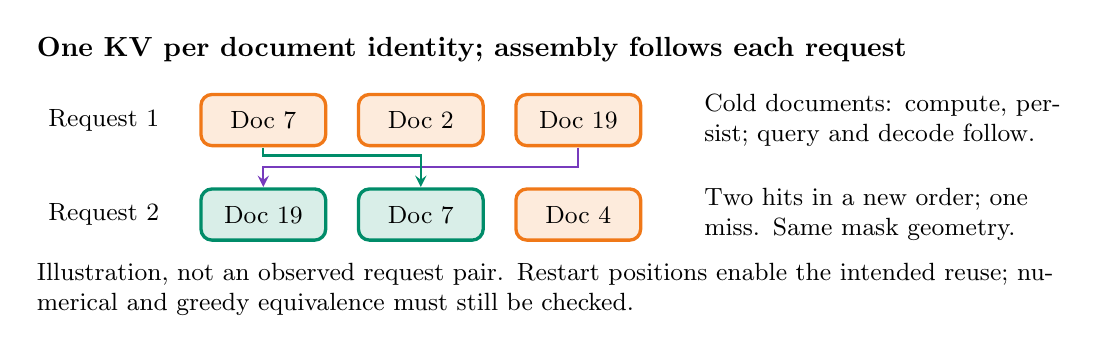
\begin{tikzpicture}[x=1cm,y=1cm,>=stealth,font=\small,
doc/.style={draw,very thick,rounded corners,text width=1.35cm,minimum height=.65cm,align=center},
note/.style={text width=4.8cm,align=left}]
\node[anchor=west,font=\bfseries] at (0,2.9)
{One KV per document identity; assembly follows each request};
\node[anchor=east] at (1.8,2) {Request 1};
\node[doc,draw=ddiGold,fill=ddiGold!15] at (3,2) {Doc 7};
\node[doc,draw=ddiGold,fill=ddiGold!15] at (5,2) {Doc 2};
\node[doc,draw=ddiGold,fill=ddiGold!15] at (7,2) {Doc 19};
\node[note] at (11,2) {Cold documents: compute, persist; query and decode follow.};
\node[anchor=east] at (1.8,.8) {Request 2};
\node[doc,draw=ddiGreen,fill=ddiGreen!15] at (3,.8) {Doc 19};
\node[doc,draw=ddiGreen,fill=ddiGreen!15] at (5,.8) {Doc 7};
\node[doc,draw=ddiGold,fill=ddiGold!15] at (7,.8) {Doc 4};
\node[note] at (11,.8) {Two hits in a new order; one miss. Same mask geometry.};
\draw[->,ddiPurple,thick] (7,1.65) -- (7,1.4) -- (3,1.4) -- (3,1.15);
\draw[->,ddiGreen,thick] (3,1.65) -- (3,1.55) -- (5,1.55) -- (5,1.15);
\node[anchor=west,text width=13cm,align=left] at (0,-.15)
{Illustration, not an observed request pair. Restart positions enable the intended reuse;
numerical and greedy equivalence must still be checked.};
\end{tikzpicture}
}
\caption{Reordering does not change which stored document identity is
requested. Hits load real KV tensors; the new document is computed.}
\label{fig:requests}
\end{figure}

Independent context processing relates to parallel context windows
\citep{ratner2023pcw}, parallel context encoding \citep{yen2024cepe}, and
Fusion-in-Decoder \citep{izacard2021fid}; here the concrete object is the
attention mask and its cached execution in a decoder-only model.

\section{The Quality Cost of Isolation}
\label{sec:quality}

Base Qwen2.5-7B-Instruct is evaluated on HotpotQA (100 records, seed 0,
greedy, batch one, bf16, A100 80GB) under four masks. Full attention
reaches EM/F1 .56/.70 against DDI-QF's .30/.42 on identical matched
requests (Table~\ref{tab:v57matched}); the isolation quality cost is real
and large. Document-count ablation shows equal EM at $N{=}10$ (.46/.46)
but persistent F1 differences; the three-seed Qwen/Llama transfer protocol
does not reach natural-QA parity (Appendix~\ref{app:quality}).

\begin{figure}[H]
\centering\resizebox{.74\linewidth}{!}{% Generated by paper/render.py; aggregates: paper/evidence.json.
% Sources: results/runs.jsonl sha256=70c098a691f9c485bd8b3ce6a3304749969f3c4d3eb4f812539bdcd867a31b47; results/sprint_c_llama.jsonl sha256=c7edb5045db9479bfcdcf403b3e38daaebf28af6fd48f14b5438000d7695ff02; results/sprint_c_1.5B.jsonl sha256=c52ef34b36b9582c88643a5a61f0ce17a87e036cfe334f23d4887808f8e23cd0; results/sprint_a_strict_base.jsonl sha256=b1196a2c1f3577c3d78b75b22d47dff7e0a14c538d428d4b0a81a1c81fa6f9fc
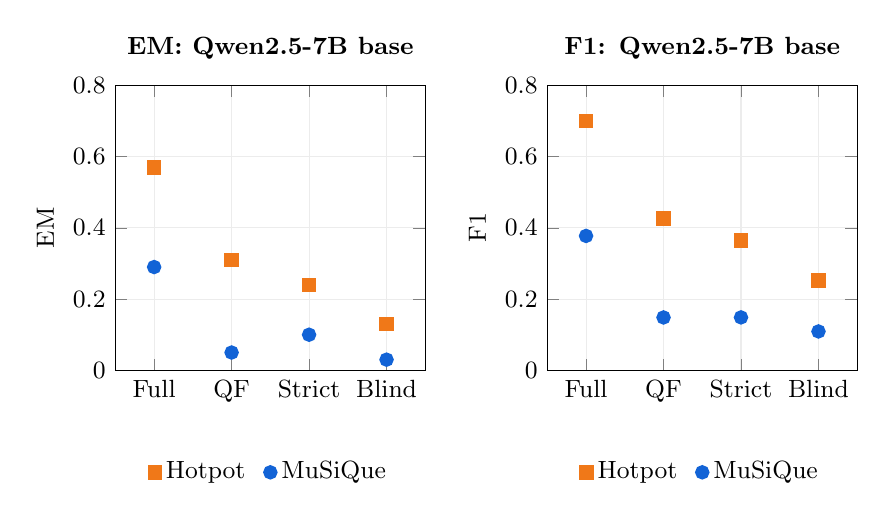
\begin{tikzpicture}
\begin{groupplot}[group style={group size=2 by 1,horizontal sep=1.55cm},width=.455\linewidth,height=5.2cm,grid=major,grid style={gray!15},tick label style={font=\small},label style={font=\small},title style={font=\small\bfseries},legend style={font=\small,draw=none,at={(.5,-.28)},anchor=north,legend columns=2,/tikz/every even column/.append style={column sep=5pt}}]
\nextgroupplot[title={EM: Qwen2.5-7B base},ylabel={EM},xtick={0,1,2,3},xticklabels={Full,QF,Strict,Blind},ymin=0,ymax=.8,xmin=-.5,xmax=3.5]
\addplot[ddiGold,very thick,mark=square*,only marks] coordinates {(0,0.570000) (1,0.310000) (2,0.240000) (3,0.130000)};
\addplot[ddiBlue,very thick,mark=*,only marks] coordinates {(0,0.290000) (1,0.050000) (2,0.100000) (3,0.030000)};
\legend{Hotpot,MuSiQue}
\nextgroupplot[title={F1: Qwen2.5-7B base},ylabel={F1},xtick={0,1,2,3},xticklabels={Full,QF,Strict,Blind},ymin=0,ymax=.8,xmin=-.5,xmax=3.5]
\addplot[ddiGold,very thick,mark=square*,only marks] coordinates {(0,0.699534) (1,0.425790) (2,0.364493) (3,0.252448)};
\addplot[ddiBlue,very thick,mark=*,only marks] coordinates {(0,0.377395) (1,0.148473) (2,0.148665) (3,0.109217)};
\legend{Hotpot,MuSiQue}
\end{groupplot}
\end{tikzpicture}
}
\caption{Quality by mask, not by numerical sparsity. Points are 100-record
means without comparison CIs.}
\label{fig:masks}
\end{figure}

\begin{figure}[H]
\centering\resizebox{.74\linewidth}{!}{% Generated by paper/render.py; aggregates: paper/evidence.json.
% Sources: results/phase3_n10.jsonl sha256=1d0a7c012582a0af40c322e6c3b91540e083ee27b2bb5a896cc9230442470dda; results/phase3_n2.jsonl sha256=1c2d4b3068468e1f76249bb1bfdc9f579797fec06f0e45b9cc8e2ef5085407c2; results/phase3_n5.jsonl sha256=6d18b180ae2df48856d304cc1184f4fbf6f76661226cd8e075eee3dea765bd34
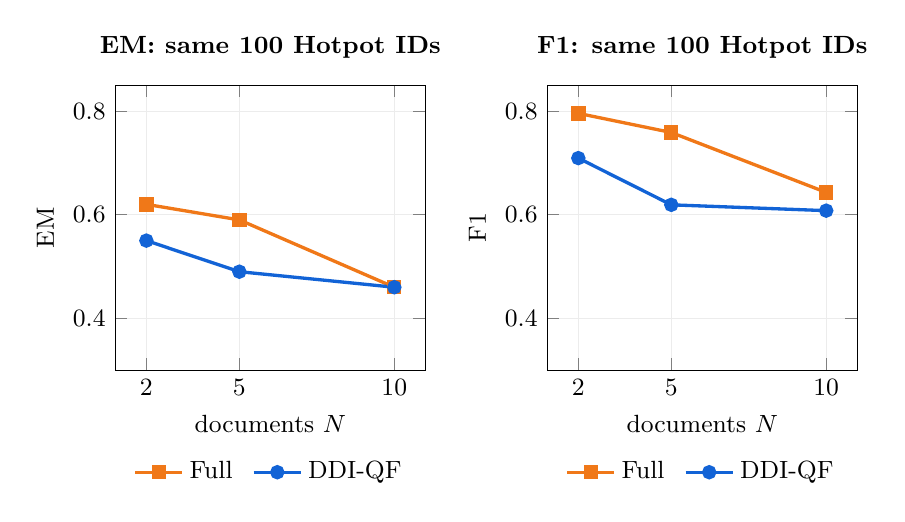
\begin{tikzpicture}
\begin{groupplot}[group style={group size=2 by 1,horizontal sep=1.55cm},width=.455\linewidth,height=5.2cm,grid=major,grid style={gray!15},tick label style={font=\small},label style={font=\small},title style={font=\small\bfseries},legend style={font=\small,draw=none,at={(.5,-.28)},anchor=north,legend columns=2,/tikz/every even column/.append style={column sep=5pt}}]
\nextgroupplot[title={EM: same 100 Hotpot IDs},xlabel={documents $N$},ylabel={EM},xtick={2,5,10},xmin=1,xmax=11,ymin=.3,ymax=.85]
\addplot[ddiGold,very thick,mark=square*] coordinates {(2,0.620000) (5,0.590000) (10,0.460000)};
\addplot[ddiBlue,very thick,mark=*] coordinates {(2,0.550000) (5,0.490000) (10,0.460000)};
\legend{Full,DDI-QF}
\nextgroupplot[title={F1: same 100 Hotpot IDs},xlabel={documents $N$},ylabel={F1},xtick={2,5,10},xmin=1,xmax=11,ymin=.3,ymax=.85]
\addplot[ddiGold,very thick,mark=square*] coordinates {(2,0.795663) (5,0.758717) (10,0.643045)};
\addplot[ddiBlue,very thick,mark=*] coordinates {(2,0.709273) (5,0.619092) (10,0.607834)};
\legend{Full,DDI-QF}
\end{groupplot}
\end{tikzpicture}
}
\caption{Document-count quality curves for one tuned checkpoint. Lines
connect three observed counts; these are not quality--sparsity curves.
Full/DDI EM is .62/.55, .59/.49, .46/.46.}
\label{fig:docquality}
\end{figure}

\begin{table}[H]
\centering\footnotesize% Generated by paper/render.py from paper/evidence.json.
% Sources: results/v57_matched_qa_hotpot100_seed0_20260908T1238Z/summary.json sha256=2cba54f3e4491feaa10496fe793e0510a27156b6f430c572c3d519d85faf88b1; results/v57_matched_qa_hotpot100_seed0_20260908T1238Z/post_audit.json sha256=1be6fd17f56003d1c4f747ff505e3557ca5b0cbec9105dc8537dbaed14bc1c7e.
% Latency ratios are means of paired per-request full/ddi_qf ratios.
\begin{tabular}{lrrl}
\toprule
 & \multicolumn{2}{c}{arm mean} & paired full $-$ ddi\_qf \\
metric & full & ddi\_qf & $\Delta$ [95\% CI] \\
\midrule
EM & 0.5600 & 0.3000 & $0.2600\;[0.1600, 0.3600]$ \\
F1 & 0.7034 & 0.4153 & $0.2881\;[0.1916, 0.3867]$ \\
presence & 0.6100 & 0.3100 & $0.3000\;[0.1900, 0.4000]$ \\
\midrule
prefill latency ratio & \multicolumn{3}{l}{$1.0013\;[1.0008, 1.0018]$} \\
request latency ratio & \multicolumn{3}{l}{$0.9955\;[0.9924, 0.9986]$} \\
\midrule
\multicolumn{4}{l}{100 matched HotpotQA requests, seed 0.} \\
\bottomrule
\end{tabular}

\caption{Matched quality and timing on identical requests (V57). The
isolation cost (.56/.70 vs .30/.42) and near-unity prefill ratio are
measured on the same records.}
\label{tab:v57matched}
\end{table}

\section{The Realization Gap: Why 95\% Sparsity Gives 0\% Speedup}
\label{sec:prefill}

For $N$ equal-length documents of $L$ tokens and a query of $Q$ tokens,
the exact prefill pair counts are $P_F = (NL{+}Q)(NL{{+}Q}{+}1)/2$ and
$P_D = NL(L{+}1)/2 + QNL + Q(Q{+}1)/2$, giving sparsity
$s = 1 - P_D/P_F$. At $N{=}25$, $L{=}512$: 95.04\% fewer pairs. Yet the
measured SDPA latency ratio is only $\sim$1.005$\times$ (Fig.~\ref{fig:prefill}).

\begin{figure}[H]
\centering\resizebox{.85\linewidth}{!}{% Generated by paper/render.py; aggregates: paper/evidence.json.
% Sources: results/runs.jsonl sha256=ca6c7a3438547933b3a78dc19bddf703b1a4c9f25a3cce5efccfaacd2880d7f9
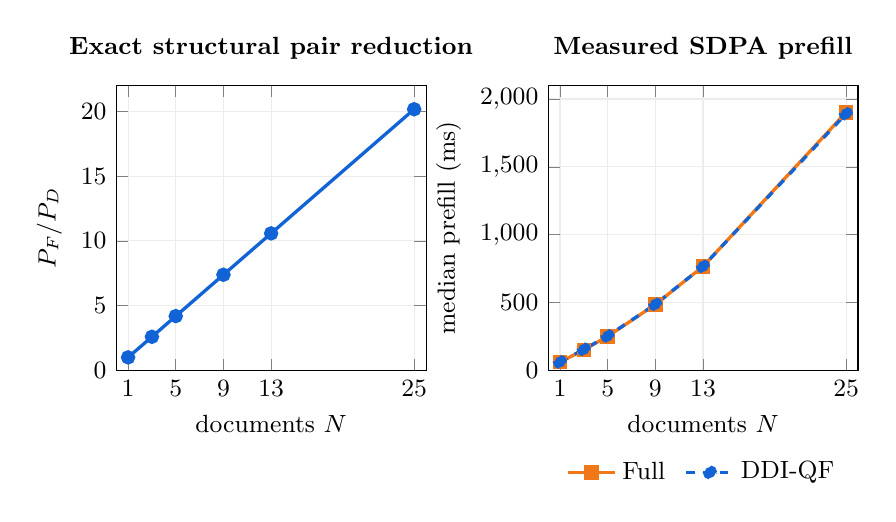
\begin{tikzpicture}
\begin{groupplot}[group style={group size=2 by 1,horizontal sep=1.55cm},width=.455\linewidth,height=5.2cm,grid=major,grid style={gray!15},tick label style={font=\small},label style={font=\small},title style={font=\small\bfseries},legend style={font=\small,draw=none,at={(.5,-.28)},anchor=north,legend columns=2,/tikz/every even column/.append style={column sep=5pt}}]
\nextgroupplot[title={Exact structural pair reduction},xlabel={documents $N$},ylabel={$P_F/P_D$},xmin=0,xmax=26,ymin=0,ymax=22,xtick={1,5,9,13,25}]
\addplot[ddiBlue,very thick,mark=*] coordinates {(1,1.000000) (3,2.590783) (5,4.186929) (9,7.381029) (13,10.575687) (25,20.160332)};
\nextgroupplot[title={Measured SDPA prefill},xlabel={documents $N$},ylabel={median prefill (ms)},xmin=0,xmax=26,ymin=0,ymax=2100,xtick={1,5,9,13,25}]
\addplot[ddiGold,very thick,mark=square*] coordinates {(1,60.351936) (3,151.028610) (5,250.308670) (9,485.391937) (13,765.888245) (25,1900.954102)};
\addplot[ddiBlue,very thick,mark=*,dashed] coordinates {(1,61.586433) (3,154.694183) (5,253.057251) (9,486.653381) (13,766.266602) (25,1891.021851)};
\legend{Full,DDI-QF}
\end{groupplot}
\end{tikzpicture}
}
\caption{Structural pair ratio (left) vs measured prefill ms (right). At
$N{=}25$: 95.04\% fewer pairs accompanies 1900.95 vs 1891.02 ms --- no
material speedup.}
\label{fig:prefill}
\end{figure}

\paragraph{Why.}
The mechanism is now measured (V101, Table~\ref{tab:dispatch}). At the
95\%-sparsity shape ($N{=}25$, $L{=}512$, $Q{=}64$), the 2D causal path
dispatches SDPA's \emph{flash} kernel, while either 4D additive mask ---
byte-equivalent full-causal or the 95\%-sparse DDI-QF --- dispatches SDPA's
\emph{memory-efficient} kernel, which reads the full bias matrix and leaves
block-sparsity unexploited: both 4D cases cost the same
($\sim$1.5$\times$ the 2D path). The block-sparse structure is invisible to
the dispatched kernel; the gap is a dispatch property, not a mask property.
Custom sparse kernels are a plausible remedy, though
Block-Attention's 98.7\% TTFT figure~\citep{ma2025blockattention}
rides on precomputed/reused document KVs and does not by itself price a
\emph{cold} sparse prefill. FlexAttention~\citep{flex_attention} compiles
block masks into sparse kernels
(historical 1.77$\times$ whole-model gain, though with older mask semantics
and unvalidated parity). The trained-contract serving path
(Section~\ref{sec:cache}) bypasses the issue entirely by reusing cached KV.

\begin{table}[H]
\centering\footnotesize% Generated by paper/render.py from paper/evidence.json.
% Sources: results/v101_sdpa_dispatch_20260915T212816Z/summary.json sha256=33eaf37cbc4781fcced6b35c18598ecf81e3f071fc511673b6a45df0fa23a7e2.
\resizebox{\linewidth}{!}{%
\begin{tabular}{llr}
\toprule
Prefill mask & Dispatched kernel & wall s / forward \\
\midrule
2d\_causal\_hf\_default & SDPA \emph{flash} & 1.889 \\
4d\_additive\_full\_causal & SDPA \emph{memory-efficient} (cutlass) & 2.829 \\
4d\_additive\_ddi\_qf & SDPA \emph{memory-efficient} (cutlass) & 2.869 \\
\midrule
\multicolumn{3}{p{0.97\linewidth}}{\footnotesize $N{=}25$, $L{=}512$, $Q{=}64$ (12{,}809 tokens; 95.86\% causal-pair sparsity), bf16, batch 1, 3 warmup + 10 profiled forwards. Block-sparsity is invisible to the dispatched kernel in every case: the 4D additive mask changes the kernel (flash $\to$ memory-efficient) and costs $\sim$1.5$\times$, not the work.} \\
\bottomrule
\end{tabular}}

\caption{SDPA kernel dispatch and wall time per prefill forward at the
95\%-sparsity shape (V101). The 4D additive mask trades flash for the
memory-efficient kernel; sparsity changes nothing.}
\label{tab:dispatch}
\end{table}

\begin{figure}[H]
\centering\resizebox{.74\linewidth}{!}{% Generated by paper/render.py; aggregates: paper/evidence.json.
% Sources: logs/timing_flex2.log sha256=2d61e4a52ba9af2aa41cbbc6532fd6f21026475a09c5d781c2702fc01eff4fd7; logs/timing_flex_model3.log sha256=a67edb5e970640a50662499717b2014328ef5a5b3ea034f2773824ba16061653
\begin{minipage}{\linewidth}\centering
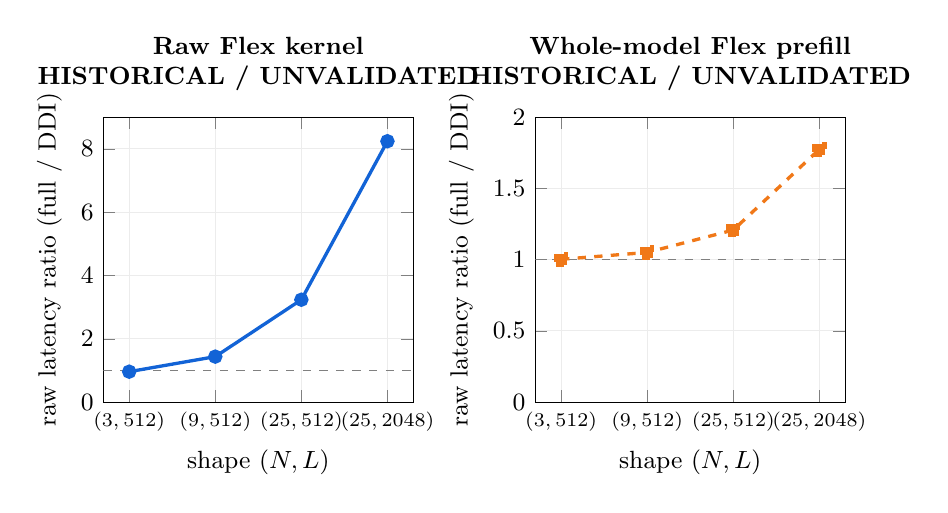
\begin{tikzpicture}
\begin{groupplot}[group style={group size=2 by 1,horizontal sep=1.55cm},width=.455\linewidth,height=5.2cm,grid=major,grid style={gray!15},tick label style={font=\small},label style={font=\small},title style={font=\small\bfseries},legend style={font=\small,draw=none,at={(.5,-.28)},anchor=north,legend columns=2,/tikz/every even column/.append style={column sep=5pt}}]
\nextgroupplot[title={Raw Flex kernel\\HISTORICAL / UNVALIDATED},title style={align=center,font=\small\bfseries},xlabel={shape $(N,L)$},ylabel={raw latency ratio (full / DDI)},xtick={0,1,2,3},xticklabels={{$(3,512)$},{$(9,512)$},{$(25,512)$},{$(25,2048)$}},x tick label style={font=\scriptsize},xmin=-.3,xmax=3.3,ymin=0,ymax=9]
\addplot[gray,dashed] coordinates {(-0.3,1.000000) (3.3,1.000000)};
\addplot[ddiBlue,very thick,mark=*] coordinates {(0,0.962406) (1,1.437776) (2,3.235775) (3,8.242600)};
\nextgroupplot[title={Whole-model Flex prefill\\HISTORICAL / UNVALIDATED},title style={align=center,font=\small\bfseries},xlabel={shape $(N,L)$},ylabel={raw latency ratio (full / DDI)},xtick={0,1,2,3},xticklabels={{$(3,512)$},{$(9,512)$},{$(25,512)$},{$(25,2048)$}},x tick label style={font=\scriptsize},xmin=-.3,xmax=3.3,ymin=0,ymax=2]
\addplot[gray,dashed] coordinates {(-0.3,1.000000) (3.3,1.000000)};
\addplot[ddiGold,very thick,dashed,mark=square*] coordinates {(0,1.002705) (1,1.050972) (2,1.208292) (3,1.774787)};
\end{groupplot}
\end{tikzpicture}
\par\smallskip{\small Independent experiments; not a matched timing decomposition.}
\end{minipage}
}
\caption{Historical Flex timing: at $N{=}25,L{=}2048$, kernel time falls
8.24$\times$ while whole-model prefill falls only 1.77$\times$ (Amdahl
dilution). Historical/unvalidated: old mask permits bidirectional
intra-document attention.}
\label{fig:flexhistory}
\end{figure}

\begin{figure}[H]
\centering\resizebox{.60\linewidth}{!}{% Generated by paper/render.py; aggregates: paper/evidence.json.
% Sources: None (analytical illustration)
% Analytical illustration only; no measured timing inputs or fitted fractions.
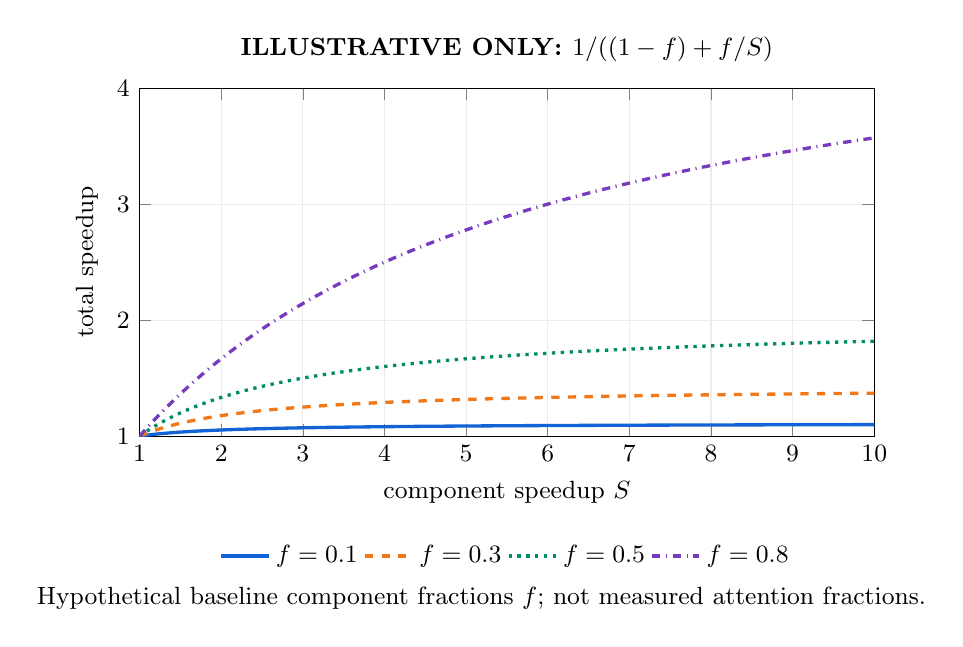
\begin{tikzpicture}
\begin{axis}[width=.9\linewidth,height=6cm,xmin=1,xmax=10,ymin=1,ymax=4,xtick={1,2,3,4,5,6,7,8,9,10},grid=major,grid style={gray!15},title={ILLUSTRATIVE ONLY: $1/((1-f)+f/S)$},title style={font=\small\bfseries},tick label style={font=\small},label style={font=\small},xlabel={component speedup $S$},ylabel={total speedup},legend style={font=\small,draw=none,at={(.5,-.28)},anchor=north,legend columns=4}]
\addplot[ddiBlue,solid,very thick,no marks] coordinates {(1.0,1.000000) (1.1,1.009174) (1.2,1.016949) (1.3,1.023622) (1.4,1.029412) (1.5,1.034483) (1.6,1.038961) (1.7,1.042945) (1.8,1.046512) (1.9,1.049724) (2.0,1.052632) (2.1,1.055276) (2.2,1.057692) (2.3,1.059908) (2.4,1.061947) (2.5,1.063830) (2.6,1.065574) (2.7,1.067194) (2.8,1.068702) (2.9,1.070111) (3.0,1.071429) (3.1,1.072664) (3.2,1.073826) (3.3,1.074919) (3.4,1.075949) (3.5,1.076923) (3.6,1.077844) (3.7,1.078717) (3.8,1.079545) (3.9,1.080332) (4.0,1.081081) (4.1,1.081794) (4.2,1.082474) (4.3,1.083123) (4.4,1.083744) (4.5,1.084337) (4.6,1.084906) (4.7,1.085450) (4.8,1.085973) (4.9,1.086475) (5.0,1.086957) (5.1,1.087420) (5.2,1.087866) (5.3,1.088296) (5.4,1.088710) (5.5,1.089109) (5.6,1.089494) (5.7,1.089866) (5.8,1.090226) (5.9,1.090573) (6.0,1.090909) (6.1,1.091234) (6.2,1.091549) (6.3,1.091854) (6.4,1.092150) (6.5,1.092437) (6.6,1.092715) (6.7,1.092985) (6.8,1.093248) (6.9,1.093502) (7.0,1.093750) (7.1,1.093991) (7.2,1.094225) (7.3,1.094453) (7.4,1.094675) (7.5,1.094891) (7.6,1.095101) (7.7,1.095306) (7.8,1.095506) (7.9,1.095700) (8.0,1.095890) (8.1,1.096076) (8.2,1.096257) (8.3,1.096433) (8.4,1.096606) (8.5,1.096774) (8.6,1.096939) (8.7,1.097100) (8.8,1.097257) (8.9,1.097411) (9.0,1.097561) (9.1,1.097708) (9.2,1.097852) (9.3,1.097993) (9.4,1.098131) (9.5,1.098266) (9.6,1.098398) (9.7,1.098528) (9.8,1.098655) (9.9,1.098779) (10.0,1.098901)};
\addplot[ddiGold,dashed,very thick,no marks] coordinates {(1.0,1.000000) (1.1,1.028037) (1.2,1.052632) (1.3,1.074380) (1.4,1.093750) (1.5,1.111111) (1.6,1.126761) (1.7,1.140940) (1.8,1.153846) (1.9,1.165644) (2.0,1.176471) (2.1,1.186441) (2.2,1.195652) (2.3,1.204188) (2.4,1.212121) (2.5,1.219512) (2.6,1.226415) (2.7,1.232877) (2.8,1.238938) (2.9,1.244635) (3.0,1.250000) (3.1,1.255061) (3.2,1.259843) (3.3,1.264368) (3.4,1.268657) (3.5,1.272727) (3.6,1.276596) (3.7,1.280277) (3.8,1.283784) (3.9,1.287129) (4.0,1.290323) (4.1,1.293375) (4.2,1.296296) (4.3,1.299094) (4.4,1.301775) (4.5,1.304348) (4.6,1.306818) (4.7,1.309192) (4.8,1.311475) (4.9,1.313673) (5.0,1.315789) (5.1,1.317829) (5.2,1.319797) (5.3,1.321696) (5.4,1.323529) (5.5,1.325301) (5.6,1.327014) (5.7,1.328671) (5.8,1.330275) (5.9,1.331828) (6.0,1.333333) (6.1,1.334792) (6.2,1.336207) (6.3,1.337580) (6.4,1.338912) (6.5,1.340206) (6.6,1.341463) (6.7,1.342685) (6.8,1.343874) (6.9,1.345029) (7.0,1.346154) (7.1,1.347249) (7.2,1.348315) (7.3,1.349353) (7.4,1.350365) (7.5,1.351351) (7.6,1.352313) (7.7,1.353251) (7.8,1.354167) (7.9,1.355060) (8.0,1.355932) (8.1,1.356784) (8.2,1.357616) (8.3,1.358429) (8.4,1.359223) (8.5,1.360000) (8.6,1.360759) (8.7,1.361502) (8.8,1.362229) (8.9,1.362940) (9.0,1.363636) (9.1,1.364318) (9.2,1.364985) (9.3,1.365639) (9.4,1.366279) (9.5,1.366906) (9.6,1.367521) (9.7,1.368124) (9.8,1.368715) (9.9,1.369295) (10.0,1.369863)};
\addplot[ddiGreen,dotted,very thick,no marks] coordinates {(1.0,1.000000) (1.1,1.047619) (1.2,1.090909) (1.3,1.130435) (1.4,1.166667) (1.5,1.200000) (1.6,1.230769) (1.7,1.259259) (1.8,1.285714) (1.9,1.310345) (2.0,1.333333) (2.1,1.354839) (2.2,1.375000) (2.3,1.393939) (2.4,1.411765) (2.5,1.428571) (2.6,1.444444) (2.7,1.459459) (2.8,1.473684) (2.9,1.487179) (3.0,1.500000) (3.1,1.512195) (3.2,1.523810) (3.3,1.534884) (3.4,1.545455) (3.5,1.555556) (3.6,1.565217) (3.7,1.574468) (3.8,1.583333) (3.9,1.591837) (4.0,1.600000) (4.1,1.607843) (4.2,1.615385) (4.3,1.622642) (4.4,1.629630) (4.5,1.636364) (4.6,1.642857) (4.7,1.649123) (4.8,1.655172) (4.9,1.661017) (5.0,1.666667) (5.1,1.672131) (5.2,1.677419) (5.3,1.682540) (5.4,1.687500) (5.5,1.692308) (5.6,1.696970) (5.7,1.701493) (5.8,1.705882) (5.9,1.710145) (6.0,1.714286) (6.1,1.718310) (6.2,1.722222) (6.3,1.726027) (6.4,1.729730) (6.5,1.733333) (6.6,1.736842) (6.7,1.740260) (6.8,1.743590) (6.9,1.746835) (7.0,1.750000) (7.1,1.753086) (7.2,1.756098) (7.3,1.759036) (7.4,1.761905) (7.5,1.764706) (7.6,1.767442) (7.7,1.770115) (7.8,1.772727) (7.9,1.775281) (8.0,1.777778) (8.1,1.780220) (8.2,1.782609) (8.3,1.784946) (8.4,1.787234) (8.5,1.789474) (8.6,1.791667) (8.7,1.793814) (8.8,1.795918) (8.9,1.797980) (9.0,1.800000) (9.1,1.801980) (9.2,1.803922) (9.3,1.805825) (9.4,1.807692) (9.5,1.809524) (9.6,1.811321) (9.7,1.813084) (9.8,1.814815) (9.9,1.816514) (10.0,1.818182)};
\addplot[ddiPurple,dashdotted,very thick,no marks] coordinates {(1.0,1.000000) (1.1,1.078431) (1.2,1.153846) (1.3,1.226415) (1.4,1.296296) (1.5,1.363636) (1.6,1.428571) (1.7,1.491228) (1.8,1.551724) (1.9,1.610169) (2.0,1.666667) (2.1,1.721311) (2.2,1.774194) (2.3,1.825397) (2.4,1.875000) (2.5,1.923077) (2.6,1.969697) (2.7,2.014925) (2.8,2.058824) (2.9,2.101449) (3.0,2.142857) (3.1,2.183099) (3.2,2.222222) (3.3,2.260274) (3.4,2.297297) (3.5,2.333333) (3.6,2.368421) (3.7,2.402597) (3.8,2.435897) (3.9,2.468354) (4.0,2.500000) (4.1,2.530864) (4.2,2.560976) (4.3,2.590361) (4.4,2.619048) (4.5,2.647059) (4.6,2.674419) (4.7,2.701149) (4.8,2.727273) (4.9,2.752809) (5.0,2.777778) (5.1,2.802198) (5.2,2.826087) (5.3,2.849462) (5.4,2.872340) (5.5,2.894737) (5.6,2.916667) (5.7,2.938144) (5.8,2.959184) (5.9,2.979798) (6.0,3.000000) (6.1,3.019802) (6.2,3.039216) (6.3,3.058252) (6.4,3.076923) (6.5,3.095238) (6.6,3.113208) (6.7,3.130841) (6.8,3.148148) (6.9,3.165138) (7.0,3.181818) (7.1,3.198198) (7.2,3.214286) (7.3,3.230088) (7.4,3.245614) (7.5,3.260870) (7.6,3.275862) (7.7,3.290598) (7.8,3.305085) (7.9,3.319328) (8.0,3.333333) (8.1,3.347107) (8.2,3.360656) (8.3,3.373984) (8.4,3.387097) (8.5,3.400000) (8.6,3.412698) (8.7,3.425197) (8.8,3.437500) (8.9,3.449612) (9.0,3.461538) (9.1,3.473282) (9.2,3.484848) (9.3,3.496241) (9.4,3.507463) (9.5,3.518519) (9.6,3.529412) (9.7,3.540146) (9.8,3.550725) (9.9,3.561151) (10.0,3.571429)};
\legend{$f=0.1$,$f=0.3$,$f=0.5$,$f=0.8$}
\end{axis}
\node[anchor=north,align=center,font=\small] at (current bounding box.south) {Hypothetical baseline component fractions $f$; not measured attention fractions.};
\end{tikzpicture}
}
\caption{Amdahl illustration: at $f{=}.1$, a 2$\times$ component speedup
gives only 1.053$\times$ overall. KV reuse avoids the document forward, not
only attention.}
\label{fig:amdahl}
\end{figure}

Segmented causal attention (V61) passes the material-speed gate in two of
eight cells: \textbf{1.118$\times$} at $N{=}5,L{=}512$ and
\textbf{1.287$\times$} at $N{=}10,L{=}512$; short shapes regress under
fixed kernel overhead. The sparse cold-path win is real but
long-document-scoped.

\section{Warm-Path Reuse: From Failed Gates to Lossless Win}
\label{sec:cache}

\paragraph{The diagnostic with failed gates (V53).}
The exact-work V53 diagnostic (50 requests, 3 seeds, $N{=}5,L{=}500$)
measured 94.53\% cache hits and 1.19$\times$ QPS ratio, but greedy IDs
differ in 19/150 streams and all numerical checks fail $10^{-4}$. The
failed gates stay visible.

\begin{center}
\fcolorbox{ddiRed}{ddiRed!6}{\parbox{.94\linewidth}{
\textbf{Failed gates remain visible.} 25/192 greedy-ID comparisons differ;
all 192/192 numerical checks fail $10^{-4}$. Not clean-revision evidence.}}
\end{center}

\begin{figure}[H]
\centering\resizebox{.76\linewidth}{!}{% Generated by paper/render.py; aggregates: paper/evidence.json.
% Sources: VIBEQUEUE-53-REPORT.md sha256=7cd9223e128c5d82b61e59575035fe4bb54c9f48c5da721723fd5d214d85195e; results/cache_v53_local_20260907/summary.json sha256=28ae886d9dae851ed090b7ebb0744b33926060d9499c3f16a01221810a0e2189; results/cache_v53_local_20260907/timing.jsonl sha256=055cf47312269ca147c6d4517d26b82aabc910b11fd6ca07f5eba5e3f54153a8; results/cache_v53_local_20260907/validation.jsonl sha256=8597c0b5394b4b17248065ad1ebc386a0a2d864f089f8e65d51d5e293f7b8d4a
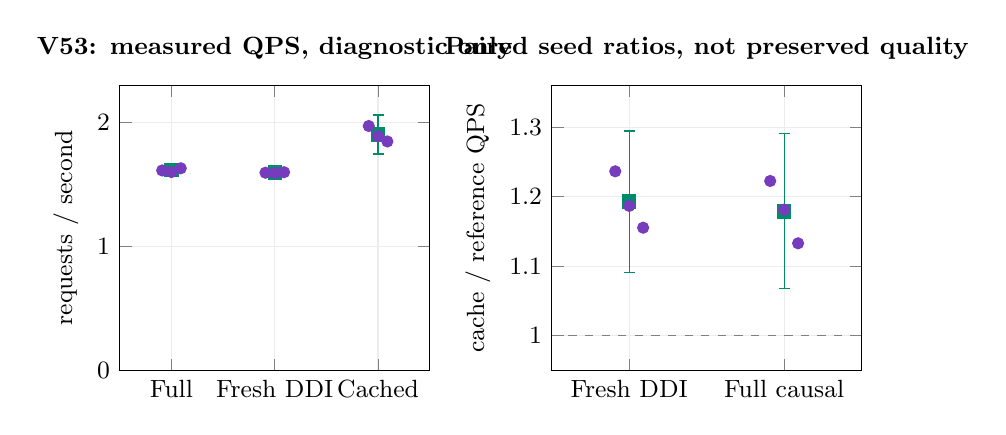
\begin{tikzpicture}
\begin{groupplot}[group style={group size=2 by 1,horizontal sep=1.55cm},width=.455\linewidth,height=5.2cm,grid=major,grid style={gray!15},tick label style={font=\small},label style={font=\small},title style={font=\small\bfseries},legend style={font=\small,draw=none,at={(.5,-.28)},anchor=north,legend columns=2,/tikz/every even column/.append style={column sep=5pt}}]
\nextgroupplot[title={V53: measured QPS, diagnostic only},ylabel={requests / second},xtick={0,1,2},xticklabels={Full,Fresh DDI,Cached},xmin=-.5,xmax=2.5,ymin=0,ymax=2.3]
\addplot[only marks,mark=square*,ddiGreen,very thick,error bars/.cd,y dir=both,y explicit] coordinates {(0,1.614982) +- (0,0.037995) (1,1.595920) +- (0,0.007711) (2,1.903480) +- (0,0.157465)};
\addplot[only marks,mark=*,ddiPurple] coordinates {(-0.09,1.613400) (0.0,1.600539) (0.09,1.631006) (0.91,1.595253) (1.0,1.593203) (1.09,1.599303) (1.91,1.972357) (2.0,1.890489) (2.09,1.847594)};
\nextgroupplot[title={Paired seed ratios, not preserved quality},ylabel={cache / reference QPS},xtick={0,1},xticklabels={Fresh DDI,Full causal},xmin=-.5,xmax=1.5,ymin=.95,ymax=1.36]
\addplot[gray,dashed] coordinates {(-.5,1) (1.5,1)};
\addplot[only marks,mark=square*,ddiGreen,very thick,error bars/.cd,y dir=both,y explicit] coordinates {(0,1.192746) +- (0,0.101649) (1,1.178812) +- (0,0.111517)};
\addplot[only marks,mark=*,ddiPurple] coordinates {(-0.09,1.236391) (0.0,1.186596) (0.09,1.155249) (0.91,1.222485) (1.0,1.181157) (1.09,1.132794)};
\end{groupplot}
\end{tikzpicture}
}
\caption{V53 QPS and paired seed ratios, diagnostic only. Not a
correctness-preserving speedup: 19/150 request pairs change outputs.}
\label{fig:qps}
\end{figure}

\paragraph{The audited warm-path win (V58--V65).}
A five-step program rebuilt the reuse path on matched natural-QA requests.
V58 measured cache-vs-fresh on 100 HotpotQA records (1.093$\times$
speedup, but exact and QA gates failed). V60 introduced a canonical
per-document encoder achieving bitwise cold/hit agreement. V65 optimized
overheads and re-ran against the monolithic baseline:

\begin{table}[H]
\centering\footnotesize% Generated by paper/render.py from paper/evidence.json.
% Sources: results/v65_benchmark_20260910T101710Z/result.json sha256=f0be727746f7788e668d39c57d29d56df047fad8cc64641a5574ea9bdcfac3a5; results/v65_combined_20260910T102918Z/result.json sha256=1edacd6a725fe922ba18897db5a6fa73272e52e54bd5e4dbdb86274c6fdff5ab.
\begin{tabular}{llr}
\toprule
Stage & Arm / contrast & TTFT median (ms) [95\% CI] \\
\midrule
benchmark & A monolithic & $127.52\;[113.45, 145.11]$ \\
benchmark & B canonical fresh & $417.42\;[413.10, 429.85]$ \\
benchmark & C all-hit reuse & $62.30\;[61.29, 64.32]$ \\
\midrule
combined & A monolithic & $127.62\;[112.66, 144.98]$ \\
combined & all-hit reuse & $58.78\;[57.83, 59.35]$ \\
combined & mixed-hit & $386.36\;[368.31, 399.28]$ \\
\midrule
ratio & benchmark C/A & $0.4885\;[0.4327, 0.5504]$ \\
ratio & benchmark B/A & $3.2735\;[2.9298, 3.6810]$ \\
ratio & combined A/all-hit & $2.1713\;[1.9428, 2.4366]$ \\
ratio & combined A/mixed-hit & $0.3303\;[0.2993, 0.3615]$ \\
\midrule
\multicolumn{3}{l}{Arm outputs byte-identical to the V60 retained generations: A 24/24, C 24/24.} \\
\multicolumn{3}{l}{End-to-end schedule walls: A 7.479 s, all-hit 5.216 s.} \\
\bottomrule
\end{tabular}

\caption{Audited warm-path result (V65, seed 47, bootstrap CIs). All-hit
reuse: 2.05$\times$ TTFT, byte-identical on 24 frozen records, 1.43$\times$
end-to-end. Mixed-hit traffic remains slower. Cold canonical prefill is
3.27$\times$ slower than monolithic.}
\label{tab:v65serving}
\end{table}

V66 measured the serving boundary on a frozen development grid:

\begin{table}[H]
\centering\footnotesize% Generated by paper/render.py from paper/evidence.json.
% Sources: results/v66_boundary_20260910T132922Z/summary.json sha256=3a4752465fe6cf0ec7b326e1a6f7108b5401dad588792188bf331f70b5a4a215; results/v66_boundary_20260910T132922Z/t9_followup_evidence_fragment.json sha256=8e25ccea000ceddeebed639c826ac22f349666dddcd9b4ba8a1559eca8d74316; results/v66_boundary_20260910T132922Z/crossover_table.md sha256=4abaab2e92530cc88e7b94efa4d905a3d58017b82a53d4211a64ee42ae80fa0e; results/v66_boundary_20260910T132922Z/scoping_sentence.md sha256=b1d836a94f2d2570cc794c793abe3bf4330e04a5d0ad1f80f1f3a25c92772cce; results/v66_boundary_20260910T132922Z/manifest.json sha256=ef217f17d2107b32039798a9d4e5a948ff063b2648145cbb310531c6a23b7779; experiments/v66_boundary_preregistration.json sha256=b6654e8e88b24b18d8076a388a9c72ed8a5ef3d1049cb382ed201fa5017afe3b.
\begin{tabular}{llr}
\toprule
Document length & Decode budget & Crossover hit fraction $h$ (wall / TTFT) \\
\midrule
L=32 & TTFT-only (d=1) & none in grid / none in grid \\
L=32 & d=8 & none in grid / none in grid \\
L=32 & d=16 & none in grid / none in grid \\
L=32 & d=32 & none in grid / none in grid \\
L=32 & d=64 & none in grid / none in grid \\
L=128 & TTFT-only (d=1) & $1$ / $0.9$ \\
L=128 & d=8 & $1$ / $0.9$ \\
L=128 & d=16 & $1$ / $0.9$ \\
L=128 & d=32 & none in grid / $0.9$ \\
L=128 & d=64 & none in grid / $0.9$ \\
L=512 & TTFT-only (d=1) & $0.7$ / $0.7$ \\
L=512 & d=8 & $0.7$ / $0.7$ \\
L=512 & d=16 & $0.8$ / $0.7$ \\
L=512 & d=32 & $0.8$ / $0.7$ \\
L=512 & d=64 & $0.8$ / $0.7$ \\
\midrule
\multicolumn{3}{l}{Development data (frozen V62 split, seed 47, single seed): outputs byte-identical on 2775/3600 timed repeats.} \\
\multicolumn{3}{l}{Headline all-hit TTFT speedup (L=512, N=10, h=1 (all-hit)): $4.28\;[4.16, 4.41]$; the all-hit wall speedup dilutes from $2.90\times$ (d=1) to $1.22\times$ (d=64).} \\
\multicolumn{3}{l}{The 825 divergent repeats are bf16 reduction-order flips deeper in the trajectory; the first decoded token is always identical.} \\
\bottomrule
\end{tabular}

\caption{Serving boundary (V66). Frozen V62 dev split, seed 47, 15 timed
repeats per cell. Cells give the smallest tested winning configuration per
shape as $h_{\mathrm{eff}}{=}$hit\_count$/N$ (wall at each decode budget and
TTFT); nominal grid labels are retained in the ledger. Development data
only; grid-specific boundaries, not universal thresholds.}
\label{tab:v66boundary}
\end{table}

\begin{table}[H]
\centering\footnotesize% Generated by paper/render.py from paper/evidence.json.
% Sources: results/v59_ttft_grid_20260908T131148Z/summary.json sha256=841b49da77af2df1ef89339b0b0182a224144a61129d0e0710d50a2fdd17cb28; results/v59_ttft_grid_20260908T131148Z/analysis.json sha256=ae69953448685c38c2e1d2653d5d765b34ac43f40e9c8ec6451265a9f4445224.
\begin{tabular}{rrcccc}
\toprule
 & & \multicolumn{2}{c}{TTFT median (ms)} & warm speedup & hit-rate \\
$N$ & $L$ & fresh & warm & [95\% CI] & crossover \\
\midrule
2 & 32 & 23.3 & 32.8 & $0.716\;[0.706, 0.731]$ & none \\
2 & 128 & 38.7 & 37.6 & $1.017\;[0.994, 1.032]$ & none \\
2 & 512 & 103.1 & 55.8 & $1.850\;[1.824, 1.864]$ & 0.733 \\
5 & 32 & 29.2 & 46.0 & $0.633\;[0.604, 0.652]$ & none \\
5 & 128 & 67.4 & 59.5 & $1.147\;[1.107, 1.200]$ & 0.955 \\
5 & 512 & 253.9 & 110.0 & $2.254\;[2.138, 2.349]$ & 0.700 \\
10 & 32 & 40.2 & 67.9 & $0.590\;[0.579, 0.600]$ & none \\
10 & 128 & 122.7 & 91.2 & $1.363\;[1.328, 1.406]$ & 0.913 \\
10 & 512 & 591.5 & 223.5 & $2.635\;[2.604, 2.662]$ & 0.616 \\
\bottomrule
\end{tabular}

\caption{TTFT geometry crossover (V59). Reuse loses at 32-token documents,
needs high hit rates at 128, wins at 512.}
\label{tab:v59crossover}
\end{table}

\paragraph{Anatomy of residual divergences (V68).}
A preregistered classification of the 22 differing records in the $n{=}100$
confirmation finds 8 near-tie flips, 11 semantic changes, 3 truncation
artifacts; bidirectional (loses EM on 5, gains on 4). The pattern is
consistent with low-magnitude bf16 reduction-order perturbation; the
classification is behavioral and does not by itself identify the numerical
root cause (Table~\ref{tab:v68anatomy}).

\begin{table}[H]
\centering\footnotesize% Generated by paper/render.py from paper/evidence.json.
% Sources: results/v68_anatomy_20260910T131036Z/anatomy_table.md sha256=68119f401e12309d534bccd43009c9d470ca73828bc28efcfcb0f0e716c2dc99; results/v68_anatomy_20260910T131036Z/classifications.jsonl sha256=9403c2af47dfb5da0436c567c193a90bfc69c24d1bf5386a78cb826170a26ee6; results/v68_anatomy_20260910T131036Z/interpretation.md sha256=f744ff9d177d2105d795501b4916c150d22911623b111f527530f1d86043002f; results/v68_anatomy_20260910T131036Z/differing_records.jsonl sha256=c7184d0ce3ef323efb8d61c472d016dfbe4640a9dfae96c1fde1eeaca5983928.
\resizebox{\linewidth}{!}{%
\begin{tabular}{lr}
\toprule
Divergence label (frozen rubric) & Records \\
\midrule
near\_tie\_greedy\_flip & 8 \\
clear\_semantic\_change & 11 \\
truncation\_stopping\_artifact & 3 \\
ambiguous & 0 \\
\midrule
\multicolumn{2}{l}{Divergence position: 9 first-token, 13 mid-generation (of 22).} \\
\multicolumn{2}{l}{Direction is two-sided: cached strictly loses EM on 5 records and strictly gains on 4, consistent with the V65 paired aggregate (EM $-0.01$).} \\
\multicolumn{2}{l}{Diagnostic only: single-seed labeled sample of 22/100 confirmation records; no rate or causal claims.} \\
\bottomrule
\end{tabular}
}

\caption{Anatomy of 22 differing cached/fresh records (V68).
Bidirectional, low-magnitude bf16 perturbation.}
\label{tab:v68anatomy}
\end{table}

\begin{figure}[H]
\centering
% Generated by paper/render.py from paper/evidence.json.
% Sources: results/v68_anatomy_20260910T131036Z/anatomy_table.md sha256=68119f401e12309d534bccd43009c9d470ca73828bc28efcfcb0f0e716c2dc99; results/v68_anatomy_20260910T131036Z/classifications.jsonl sha256=9403c2af47dfb5da0436c567c193a90bfc69c24d1bf5386a78cb826170a26ee6; results/v68_anatomy_20260910T131036Z/interpretation.md sha256=f744ff9d177d2105d795501b4916c150d22911623b111f527530f1d86043002f; results/v68_anatomy_20260910T131036Z/differing_records.jsonl sha256=c7184d0ce3ef323efb8d61c472d016dfbe4640a9dfae96c1fde1eeaca5983928.
% V18: anatomy of the 22 divergent cached/fresh confirmation records (V68).
% Counts from the pinned T16_v68_anatomy ledger artifact.
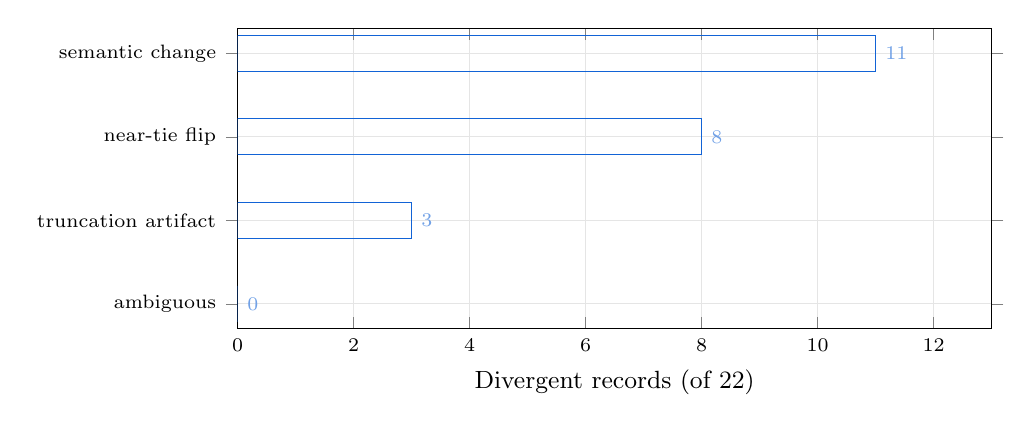
\begin{tikzpicture}
\begin{axis}[
  width=0.92\linewidth, height=5.4cm,
  xbar, bar width=13pt,
  symbolic y coords={ambiguous,truncation artifact,near-tie flip,semantic change},
  ytick=data,
  xtick={0,2,4,6,8,10,12},
  xlabel={{Divergent records (of 22)}},
  xmin=0, xmax=13,
  yticklabel style={font=\scriptsize},
  tick label style={font=\scriptsize},
  label style={font=\small},
  nodes near coords, nodes near coords align={horizontal},
  every node near coord/.append style={font=\scriptsize},
  grid=both, grid style={gray!20},
]
\addplot[ddiBlue!60, draw=ddiBlue]
  coordinates {(0,ambiguous) (3,truncation artifact) (8,near-tie flip) (11,semantic change)};
\end{axis}
\end{tikzpicture}

\caption{V68 divergence anatomy (rubric frozen before inspection). Of the
22 divergent records: 11 clear semantic changes, 8 near-tie greedy flips,
3 truncation/stopping artifacts, none ambiguous. Direction: cached
strictly gains on 4 and strictly loses on 5; position: 9 first-token,
13 mid-generation.}
\label{fig:anatomy}
\end{figure}

\begin{table}[H]
\centering\footnotesize% Generated by paper/render.py from paper/evidence.json.
% Sources: results/v60_confirmation24_20260910T093500Z/result.json sha256=9421b268eefaf7fcf6bc60b80469ba43a8b6868f9c0dfec123647ff259547464; results/v60_confirmation24_20260910T093500Z/requests.jsonl sha256=ec08d056d6ebe9208cf831e8a63e2d527cc8afec90d377ad9356635767410a5c; results/v64_audit_20260910T091231Z_QA_RECOMPUTATION/recomputation.json sha256=7850dbd4664ac50ff2f8d4f7d8de5420441bdb31da86d04aad7f2d911174fb63; results/v65_combined_20260910T102918Z/result.json sha256=1edacd6a725fe922ba18897db5a6fa73272e52e54bd5e4dbdb86274c6fdff5ab.
\begin{tabular}{llrrl}
\toprule
Cohort & Metric & $\Delta$ mean & 95\% CI & Verdict \\
\midrule
V64 (n=24) & EM & +0.041667 & $[-0.083333, 0.166667]$ & inconclusive \\
V64 (n=24) & F1 & +0.021982 & $[-0.070833, 0.119518]$ & inconclusive \\
\midrule
V65 (n=100) & EM & -0.0100 & $[-0.0700, 0.0500]$ & not non-inferior \\
V65 (n=100) & F1 & -0.0095 & $[-0.0527, 0.0312]$ & not non-inferior \\
\midrule
\multicolumn{5}{l}{Non-inferiority floor: 95\% CI lower bound $\geq -0.02$ for both EM and F1.} \\
\multicolumn{5}{l}{V65 untouched: prediction-equal 78/100, first-token-equal 91/100.} \\
\bottomrule
\end{tabular}

\caption{QA non-inferiority under the $-0.02$ floor (paired bootstrap,
seed 47). The 100-record confirmation fails under the \emph{untrained}
contract; the trained contract is in Table~\ref{tab:v70gates}.}
\label{tab:qaconfirmation}
\end{table}

\paragraph{The final trained contract (specification).}
The production contract is a $k{=}5$ fixed-marker link-token layout with a
top-8-layer self-distilled checkpoint. The five marker embeddings are fixed
deterministic vectors (not learned); link rows are reachable from answer
rows, and every document begins at a restart position (position index zero)
while the physical KV layout stores documents in original order --- the
logical attention layout and the physical cache layout are related but
distinct objects, and cache identity covers checkpoint, tokenizer, layout,
and exact token content. Only the top 8 decoder layers are trainable.
Training minimizes a self-distillation loss against a frozen teacher that
always executes the no-link, sequential, full-causal path: each record
presentation uses the differentiable independently encoded bf16 document
K/V path with probability 15\% and monolithic encoding with 85\%, on a
SHA-256 arm-independent schedule. Optimization: effective batch 4 (four
accumulated backwards per step), learning rate $10^{-5}$ after a 20-step
linear warmup, 1{,}000 optimizer steps $=$ 4{,}000 presentations $=$ 5
epochs over the frozen 800-record train split, bf16, 6-hour wall cap.
Development selection maximizes persisted-C EM then F1 between $k{=}0$ and
$k{=}5$ on a frozen 100-record dev split; confirmation and development IDs
are disjoint. Generation at evaluation: greedy, batch one,
\texttt{max\_new\_tokens} ${=} 64$, EOS from the tokenizer.

\paragraph{Quality arms (V70/V72).}
All four arms below run on the \emph{same trained checkpoint}; none of them
is the original untrained model.
\begin{itemize}
\item \textbf{A (diagnostic):} monolithic generation with the trained
contract's link layout on the trained weights.
\item \textbf{B (fresh reference):} independent per-document canonical
encoding in memory, then the shared greedy callable.
\item \textbf{C (persisted, gated):} identical callable, with document
entries read from a reopened persisted store --- hit-only, fail-closed on
any encode attempt, keys and entry counts unchanged.
\item \textbf{D (diagnostic):} trained weights under a full-causal mask with
no links; per the harness this changes the mask while retaining the restart
positions and physical link layout of the contract.
\end{itemize}

\paragraph{Cache fidelity is exact (V70, V72).}
Per record, the harness asserts B and C document K/V tensors are equal
(shape, dtype, detached-CPU comparison) before generation, and B/C outputs
are then produced by the same greedy callable on identical inputs --- so
cached-vs-fresh execution identity is a property of canonical execution and
persistence correctness, \emph{not} a training effect. The data agree: C$-$B
is exactly zero on EM and F1 at all three stations. The percentile-bootstrap
interval for an all-zero paired difference is degenerate $[0,0]$ --- every
resample returns zero --- so the interval adds no information beyond the
point mass, and we do not present it as independent confirmation. The
stations differ in dev-selected arm: $k{=}5$ at seed 47 (V70), $k{=}0$ at
seed 1 (V72-a), and $k{=}5$ on Llama-3.1-8B (V72-b; $n{=}300$ each,
$\max_{\text{new}}{=}64$). Identity holds at every station regardless of
$k$, which is exactly the claim: it is contract-level execution fidelity,
not a $k{=}5$ training outcome. The three stations reuse the same frozen
300 confirmation records, so they replicate the \emph{property} across
seeds and families; they are not independent new request samples.

\paragraph{Confirmation provenance.}
The confirmation300 split contains the original V62 confirmation100 as
positions 1--100 (SHA-pinned in the verdict); its 22 divergent records were
subsequently classified in V68. ``Untouched'' therefore means untouched by
training and by selection --- selection read record IDs only, never labels,
predictions, or metrics --- not never-before-evaluated. V68's divergence
inspection happened after the V62 evaluation and before the V70/V72
confirmations; no gate, margin, or treatment was changed in response to it,
and the V68 population is reported post hoc only
(experiments/v70\_preregistration.md, amendments 1--3).
\paragraph{Within-contract quality contrasts (V110 decomposition).}
The gated contrast C$-$D (isolated cached vs.\ the V70 D construction) passes
non-inferiority with large margins (EM $+0.240$ seed 47, $+0.277$ seed 1,
$+0.123$ Llama), and V110 now explains the D side of that gap. Decomposing
the D arm on the trained $k{=}5$ checkpoint (Table~\ref{tab:arms}): a plain
sequential stream under a full-causal mask scores EM 0.4533
($k5$-std), the same plain stream under the isolated DDI-QF mask scores EM
0.4833 ($k5$-iso-seq) --- both near the contract's cached quality --- while
the pinned D construction (full-causal mask \emph{on} the restart/link
layout) collapses to EM 0.1967 ($k5$-d-replica; the pinned run measured
0.1833 on an earlier runtime stack, deviation recorded in the prereg). In
the mask $\times$ layout grid, only the mixed cell fails: the trained
contract requires its mask and layout to cohere, and full-causal execution
itself is \emph{not} out-of-distribution for the trained weights. We report
this as a measured characterization and retract the earlier
``full-causal is out-of-distribution'' wording.

\paragraph{The original-model reference (V109).}
The matched reference the confirmations lacked: the original
Qwen2.5-7B-Instruct on the byte-identical token stream, sequential
positions, full-causal mask (Table~\ref{tab:arms}). It reaches EM 0.5533 /
F1 0.6928, so the cached contract's C arm sits $-0.130$ EM
(95\% CI $[-0.187, -0.073]$) and $-0.137$ F1 below it: the isolation-plus-
training pipeline does \emph{not} preserve original-model QA at $n{=}300$,
and we claim only what the gates support --- exact cached-vs-fresh
identity and the within-contract contrasts --- with the original-model gap
stated as measured. Even the best plain-stream variant on the trained
weights ($k5$-iso-seq, EM 0.4833) remains $-0.07$ EM below the original
model.

\begin{table}[H]
\centering\footnotesize% Generated by paper/render.py from paper/evidence.json.
% Sources: results/v109_v110_20260915T211622Z/summary.json sha256=c52ee1ccd6d0a2cbdc0accddb0fc6b8bb8dac3fda402e25a87baf537ee71b340.
\resizebox{\linewidth}{!}{%
\begin{tabular}{lrrrr}
\toprule
Arm & EM & F1 & C$-$arm EM & 95\% CI \\
\midrule
base model, full-causal, sequential (V109 R) & 0.5533 & 0.6928 & +0.1300 & $[+0.0733, +0.1867]$ \\
trained $k5$, plain stream, full-causal, sequential (V110) & 0.4533 & 0.6011 & +0.0300 & $[-0.0267, +0.0867]$ \\
trained $k5$, plain stream, isolated mask, sequential (V110) & 0.4833 & 0.5968 & +0.0600 & $[+0.0200, +0.1000]$ \\
trained $k5$, V70 D: full-causal on contract layout (V110) & 0.1967 & 0.2865 & -0.2267 & $[-0.2900, -0.1633]$ \\
\midrule
\multicolumn{5}{p{0.97\linewidth}}{\footnotesize $n{=}300$ frozen confirmation300 records, greedy 64, bf16 eager, batch 1. Paired bootstrap (10k, seed 47) against the pinned V70 C arm (EM 0.4233, F1 0.5561). The pinned V70 C/B arms run the isolated mask on the restart/link contract layout; k5-d-replica reproduces the pinned D construction (runtime drift recorded as prereg Amendment 1).} \\
\bottomrule
\end{tabular}}

\caption{Original-model reference (V109) and D-arm decomposition (V110) on
the frozen confirmation300 records, with paired C$-$arm deltas against the
pinned V70 C arm.}
\label{tab:arms}
\end{table}

To our knowledge, no prior work frames cache reuse as an exact
persisted-vs-fresh execution identity question; KVLink
\citep{yang2025kvlink} targets approximate quality recovery, CacheBlend
\citep{yao2025cacheblend} recomputes 5--18\% of tokens per layer, CacheClip
\citep{yang2025cacheclip} uses an auxiliary model for selected tokens.

\begin{table}[H]
\centering\footnotesize% Generated by paper/render.py from paper/evidence.json.
% Sources: results/v70_confirmation300_k5.json sha256=9283392c5a8669237a8152a9a884ed6045693fbc556d37aecf951eb3b07795f0; results/v70_confirmation_analysis_20260911T152345Z/verdict.json sha256=6bd916f922c233d90df9e913a01b7907b326ceb86f482231c4253f2e4ce63ddd.
\begin{tabular}{llrrl}
\toprule
Arm & Role & EM & F1 & \\
\midrule
A & diagnostic only & 0.436667 & 0.582616 \\
B & diagnostic only & 0.423333 & 0.556105 \\
C & gate candidate & 0.423333 & 0.556105 \\
D & gate reference & 0.183333 & 0.281448 \\
\midrule
Gate & Metric & $\Delta$ mean & 95\% CI & Verdict \\
C-B & EM & +0.000000 & $[0.000000, 0.000000]$ & PASS \\
C-B & F1 & +0.000000 & $[0.000000, 0.000000]$ & PASS \\
C-D & EM & +0.240000 & $[0.176667, 0.300000]$ & PASS \\
C-D & F1 & +0.274658 & $[0.211618, 0.335189]$ & PASS \\
\midrule
\multicolumn{5}{l}{300 frozen confirmation300 records; non-inferiority margin -0.02; 10000 paired bootstrap resamples, seed 47.} \\
\multicolumn{5}{l}{k=5 selected checkpoint; arms A and B are diagnostic only per the frozen verdict.} \\
\multicolumn{5}{l}{Arm C read hit-only from a reopened persisted store: 2947 entries before and after, keys unchanged, encode-on-miss fails closed.} \\
\bottomrule
\end{tabular}

\caption{Trained reuse-contract confirmation (V70, seed 47, $k{=}5$). 300
confirmation records (V62 confirmation100 included; untouched by training
and selection), paired bootstrap (10k, seed 47, margin $-0.02$). C$-$B
exactly zero (degenerate CI); C$-$D passes. A and D are diagnostics on the
same trained checkpoint.}
\label{tab:v70gates}
\end{table}

\begin{figure}[H]
\centering
% Generated by paper/render.py from paper/evidence.json.
% Sources: results/v70_confirmation_analysis_20260911T152345Z/verdict.json sha256=6bd916f922c233d90df9e913a01b7907b326ceb86f482231c4253f2e4ce63ddd; results/v72_confirmation_analysis/verdict.json sha256=c4625da0bb76ca9001e361832db0fc635aa3f55ecb81a8e3b4bbe3947765136c; results/v72s2_confirmation_analysis/verdict.json sha256=d398b260993d35337218c152d60ba4a04739cb6176320f3ce1d913eb96526ad4.
% V16: trained-contract quality gates across the three n=300 confirmations.
% C-B is exactly 0.000 with degenerate CI [0,0] at every station: the
% all-zero paired differences make every bootstrap resample zero, so the
% interval carries no information beyond the point mass (VIBEQUEUE-94).
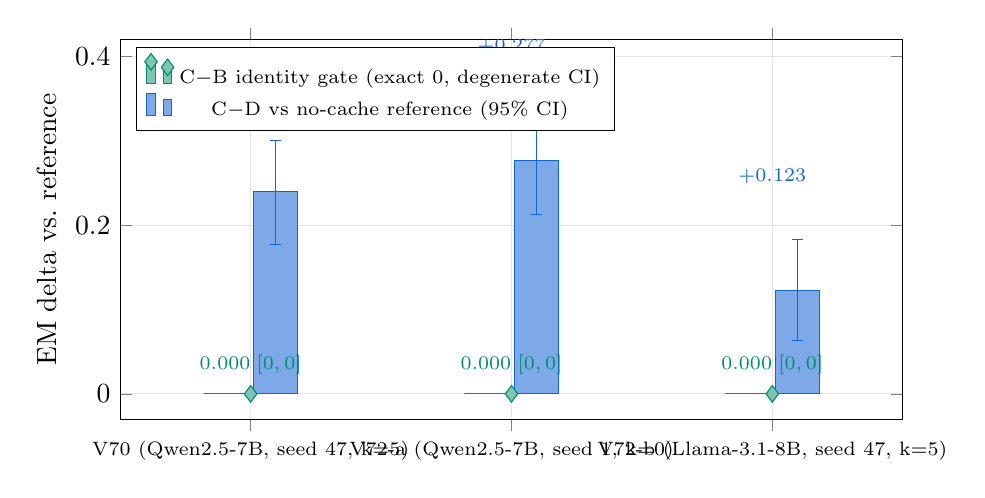
\begin{tikzpicture}
\begin{axis}[
  width=0.95\linewidth, height=6.4cm,
  ybar, bar width=16pt,
  symbolic x coords={V70,V72-a,V72-b},
  xtick=data,
  xticklabels={{V70 (Qwen2.5-7B, seed 47, k=5)},{V72-a (Qwen2.5-7B, seed 1, k=0)},{V72-b (Llama-3.1-8B, seed 47, k=5)}},
  xticklabel style={font=\scriptsize},
  ylabel={EM delta vs.\ reference},
  ymin=-0.03, ymax=0.42, enlarge x limits=0.25,
  legend style={at={(0.02,0.98)}, anchor=north west, font=\scriptsize},
  grid=both, grid style={gray!20},
]
\addplot[ddiGreen, fill=ddiGreen!50, mark=diamond*, mark size=3pt,         error bars/.cd, y dir=both, y explicit]
  coordinates {(V70,0) += (0,0) -= (0,0) (V72-a,0) += (0,0) -= (0,0) (V72-b,0) += (0,0) -= (0,0)};
\addlegendentry{C$-$B identity gate (exact $0$, degenerate CI)}
\addplot[ddiBlue, fill=ddiBlue!55,
         error bars/.cd, y dir=both, y explicit]
  coordinates {(V70,0.24) += (0,0.06) -= (0,0.063) (V72-a,0.277) += (0,0.06) -= (0,0.064) (V72-b,0.123) += (0,0.06) -= (0,0.06)};
\addlegendentry{C$-$D vs no-cache reference (95\% CI)}
\node[font=\scriptsize, ddiGreen, anchor=south] at (axis cs:V70,0.012) {$0.000\;[0,0]$};
\node[font=\scriptsize, ddiBlue, anchor=south] at (axis cs:V70,0.355) {$+0.240$};
\node[font=\scriptsize, ddiGreen, anchor=south] at (axis cs:V72-a,0.012) {$0.000\;[0,0]$};
\node[font=\scriptsize, ddiBlue, anchor=south] at (axis cs:V72-a,0.392) {$+0.277$};
\node[font=\scriptsize, ddiGreen, anchor=south] at (axis cs:V72-b,0.012) {$0.000\;[0,0]$};
\node[font=\scriptsize, ddiBlue, anchor=south] at (axis cs:V72-b,0.238) {$+0.123$};
\end{axis}
\end{tikzpicture}

\caption{Trained-contract quality gates across the three $n{=}300$
confirmations (same frozen records at every station). The identity gate
C$-$B is exactly zero at every station; its percentile-bootstrap interval
is the degenerate $[0,0]$ of an all-zero paired difference and carries no
information beyond the point (green diamonds). The no-cache deficit C$-$D
stays in the $+0.12$--$+0.28$ EM band (blue bars, 95\% paired-bootstrap
CIs, 10k resamples). Station labels give the dev-selected arm: $k{=}5$
(seed 47), $k{=}0$ (seed 1), $k{=}5$ (Llama-3.1-8B).}
\label{fig:gatedeltas}
\end{figure}

\paragraph{The trained contract keeps the serving win (V71).}
V71 measures the trained $k{=}5$ contract's serving boundary on the frozen
V66 grid (240 (shape, hit-count, budget) configurations, 15 timed repeats
each, seed 47) against four arms:

\begin{itemize}
\item \textbf{A (reference):} the \emph{untrained} restart checkpoint
(V66 pin), monolithic generation under the DDI-QF mask with restart
positions; its wall covers model forward plus fixed-work decode (mask build
untimed). A is neither the original model nor a full-causal reference; it is
the untrained-contract monolithic pricing.
\item \textbf{BP (trained fresh):} per-pass independent canonical encode on
the trained checkpoint, same callable as CP.
\item \textbf{CP (trained cached):} document entries from the canonical
store (mixed cells write through misses); CP wall additionally covers store
retrieval and entry assembly, and strict CP TTFT additionally covers
first-token selection --- both inside the timed callable, which is
conservative for CP. Request layout construction is outside the timed
region for all arms.
\item \textbf{DP (diagnostic):} trained full-causal monolithic prefill,
TTFT only.
\end{itemize}

The primary gate (A/CP paired ratio of medians, frozen V66 materiality
rule) and the secondary sanity gate (CP$\equiv$BP byte-identical per
repeat) both hold: zero divergent decodes across all 240 configurations.
The boundary improves or shifts per shape
(Table~\ref{tab:v71boundary}): the smallest tested winning configurations
reach $h_{\mathrm{eff}}{=}0.6$ (wall, $d{=}1$) and $0.7$ (TTFT) at
$L{=}512$, and $0.9$ / $1.0$ at $L{=}128$ --- per-shape grid outcomes, not
universal thresholds. All-hit TTFT reaches $5.55\times$ and all-hit wall
($d{=}1$) $6.55\times$ at $L{=}512,N{=}10$. The $5N$ link-token overhead is
invisible at $L{=}512$ ($\sim$1\% of prefill).

\begin{table}[H]
\centering\footnotesize% Generated by paper/render.py from paper/evidence.json.
% Sources: results/v71_trained_serving_v2/result.json sha256=0bd1d1a67dff133f4b51b1925edf92545900853dfecbe715154c83df3bc47301; results/v71_trained_serving_v2/summary.json sha256=af4e9bb062f1d5022e4adc49c182b2c447dd21b659571812f0dfd7e83928bd6d.
\begin{tabular}{llrrlrrl}
\toprule
budget & $L$ & V66 wall $h$ & V71 wall $h$ & shift & V66 TTFT $h$ & V71 TTFT $h$ & shift \\
\midrule
TTFT & 32 & none & none & --- & none & none & --- \\
d=8 & 32 & none & none & --- & none & none & --- \\
d=16 & 32 & none & none & --- & none & none & --- \\
d=32 & 32 & none & none & --- & none & none & --- \\
d=64 & 32 & none & none & --- & none & none & --- \\
\midrule
TTFT & 128 & none & none & --- & none & none & --- \\
d=8 & 128 & 1 & 0.9 & -0.1 & 0.9 & 0.8 & -0.1 \\
d=16 & 128 & 1 & 0.9 & -0.1 & 0.9 & 0.8 & -0.1 \\
d=32 & 128 & none & 1 & appears & 0.9 & 0.8 & -0.1 \\
d=64 & 128 & none & none & --- & 0.9 & 0.8 & -0.1 \\
\midrule
TTFT & 512 & none & none & --- & none & none & --- \\
d=8 & 512 & 0.7 & 0.6 & -0.1 & 0.7 & 0.7 & 0 \\
d=16 & 512 & 0.8 & 0.6 & -0.2 & 0.7 & 0.7 & 0 \\
d=32 & 512 & 0.8 & 0.7 & -0.1 & 0.7 & 0.7 & 0 \\
d=64 & 512 & 0.8 & 0.7 & -0.1 & 0.7 & 0.7 & 0 \\
\bottomrule
\end{tabular}

\caption{Serving boundary per shape, untrained (V66) vs.\ trained (V71)
contract, as smallest tested winning $h_{\mathrm{eff}}{=}$hit\_count$/N$
under the frozen materiality rule. Smaller is better; ---{} = none in the
frozen grid. Grid-specific, not universal thresholds.}
\label{tab:v71boundary}
\end{table}

\begin{figure}[H]
\centering
% Generated by paper/render.py from paper/evidence.json.
% Sources: results/v71_trained_serving_v2/result.json sha256=0bd1d1a67dff133f4b51b1925edf92545900853dfecbe715154c83df3bc47301; results/v66_boundary_20260910T132922Z/crossover_table.md sha256=4abaab2e92530cc88e7b94efa4d905a3d58017b82a53d4211a64ee42ae80fa0e.
\begin{tikzpicture}
\begin{groupplot}[
  group style={group size=2 by 1, horizontal sep=1.5cm},  width=0.46\linewidth, height=5.8cm,  xlabel={$h_{\mathrm{eff}}$ = hit\_count/$N$ (actual cached fraction)},  xmin=0, xmax=1.05, ymin=0,  ymax=7,  grid=both, grid style={gray!20},  title style={font=\small},  tick label style={font=\scriptsize}, label style={font=\small},]
\nextgroupplot[title={A/CP wall speedup, decode $d{=}1$}]\legend{{V66 $N{=}2$},{V66 $N{=}5$},{V66 $N{=}10$}}
\addplot[gray, dashed, no marks, domain=0:1.05] {1};
\addplot[ddiBlue, dashed, mark=*, mark size=1.5pt, mark options={solid}, forget plot] coordinates {(0,0.334) (0.5,0.524) (1,1.323)};
\addplot[ddiBlue, solid, mark=square*, mark size=1.5pt, mark options={solid}, forget plot] coordinates {(0,0.397) (0.5,0.685) (1,2.593)};
\addplot[ddiGreen, dashed, mark=*, mark size=1.5pt, mark options={solid}, forget plot] coordinates {(0,0.369) (0.2,0.419) (0.6,0.704) (0.8,1.109) (1,2.417)};
\addplot[ddiGreen, solid, mark=square*, mark size=1.5pt, mark options={solid}, forget plot] coordinates {(0,0.422) (0.2,0.535) (0.6,0.942) (0.8,1.476) (1,4.508)};
\addplot[ddiGold, dashed, mark=*, mark size=1.5pt, mark options={solid}, forget plot] coordinates {(0,0.458) (0.3,0.559) (0.5,0.737) (0.6,0.838) (0.7,1.043) (0.8,1.236) (0.9,1.692) (1,2.901)};
\addplot[ddiGold, solid, mark=square*, mark size=1.5pt, mark options={solid}, forget plot] coordinates {(0,0.494) (0.3,0.699) (0.5,0.919) (0.6,1.097) (0.7,1.37) (0.8,1.916) (0.9,2.943) (1,6.55)};
\nextgroupplot[title={A/CP TTFT speedup}]
\addplot[gray, dashed, no marks, domain=0:1.05] {1};
\addplot[ddiBlue, dashed, mark=*, mark size=1.5pt, mark options={solid}, forget plot] coordinates {(0,0.351) (0.5,0.587) (1,2.06)};
\addplot[ddiBlue, solid, mark=square*, mark size=1.5pt, mark options={solid}, forget plot] coordinates {(0,0.38) (0.5,0.654) (1,2.537)};
\addplot[ddiGreen, dashed, mark=*, mark size=1.5pt, mark options={solid}, forget plot] coordinates {(0,0.368) (0.2,0.421) (0.6,0.751) (0.8,1.201) (1,3.413)};
\addplot[ddiGreen, solid, mark=square*, mark size=1.5pt, mark options={solid}, forget plot] coordinates {(0,0.384) (0.2,0.469) (0.6,0.83) (0.8,1.379) (1,4.033)};
\addplot[ddiGold, dashed, mark=*, mark size=1.5pt, mark options={solid}, forget plot] coordinates {(0,0.424) (0.3,0.541) (0.5,0.724) (0.6,0.864) (0.7,1.055) (0.8,1.325) (0.9,2.032) (1,4.281)};
\addplot[ddiGold, solid, mark=square*, mark size=1.5pt, mark options={solid}, forget plot] coordinates {(0,0.424) (0.3,0.611) (0.5,0.803) (0.6,0.963) (0.7,1.204) (0.8,1.684) (0.9,2.534) (1,5.547)};
\end{groupplot}
\matrix [draw=none, anchor=north, font=\scriptsize, matrix of nodes, nodes={anchor=west}, row sep=1pt, column sep=10pt] at (current bounding box.south) {
\tikz\draw[ddiBlue,dashed] (0,0) -- (0.35,0); V66 $N{=}2$ & \tikz\draw[ddiBlue,solid] (0,0) -- (0.35,0); V71 $N{=}2$ \\
\tikz\draw[ddiGreen,dashed] (0,0) -- (0.35,0); V66 $N{=}5$ & \tikz\draw[ddiGreen,solid] (0,0) -- (0.35,0); V71 $N{=}5$ \\
\tikz\draw[ddiGold,dashed] (0,0) -- (0.35,0); V66 $N{=}10$ & \tikz\draw[ddiGold,solid] (0,0) -- (0.35,0); V71 $N{=}10$ \\};
\end{tikzpicture}

\caption{Serving speedup vs.\ the untrained-restart monolithic reference
(A) as a function of the actual cached fraction
$h_{\mathrm{eff}}{=}$hit\_count$/N$, at $L{=}512$. Left: end-to-end wall
speedup at decode budget $d{=}1$ (A/CP paired ratio of medians, the primary
gate metric). Right: strict TTFT speedup (A/CP first-token latency). Dashed:
untrained contract (V66); solid: trained contract (V71). The trained
contract shifts the per-shape boundaries left and reaches $6.55\times$
(wall, $d{=}1$) and $5.55\times$ (TTFT) at all-hit ($N{=}10$). Below the
break-even line (gray dashed), reuse loses.}
\label{fig:crossover512}
\end{figure}

\begin{figure}[H]
\centering
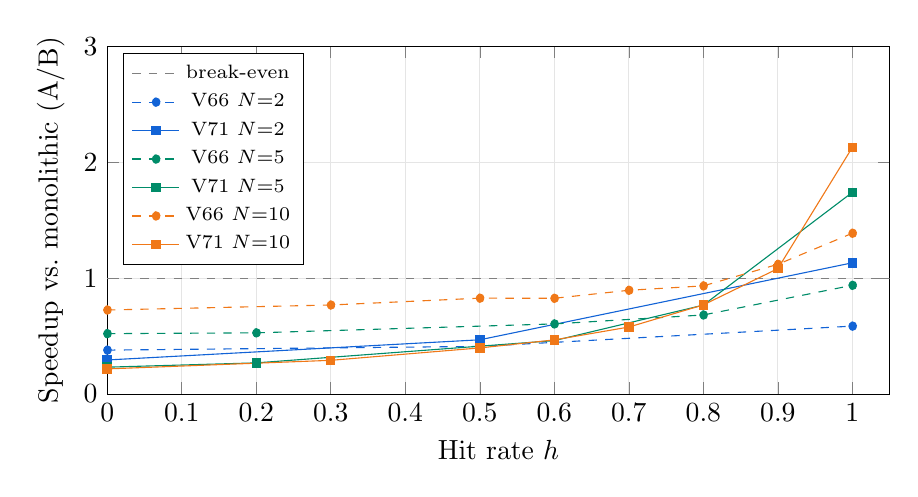
\begin{tikzpicture}
\begin{axis}[
  width=0.95\linewidth, height=6cm,
  xlabel={Hit rate $h$}, ylabel={Speedup vs.\ monolithic (A/B)},
  xmin=0, xmax=1.05, ymin=0, ymax=3,
  legend style={at={(0.02,0.98)}, anchor=north west, font=\scriptsize},
  grid=both, grid style={gray!20},
]
\addplot[gray, dashed, no marks, domain=0:1.05] {1};
\addlegendentry{break-even}
\addplot[ddiBlue, dashed, mark=*, mark size=1.5pt] coordinates {(0.00,0.379) (0.50,0.411) (1.00,0.586)};
\addlegendentry{V66 $N{=}2$}
\addplot[ddiBlue, solid, mark=square*, mark size=1.5pt] coordinates {(0.00,0.294) (0.50,0.468) (1.00,1.132)};
\addlegendentry{V71 $N{=}2$}
\addplot[ddiGreen, dashed, mark=*, mark size=1.5pt] coordinates {(0.00,0.521) (0.20,0.528) (0.60,0.605) (0.80,0.682) (1.00,0.938)};
\addlegendentry{V66 $N{=}5$}
\addplot[ddiGreen, solid, mark=square*, mark size=1.5pt] coordinates {(0.00,0.232) (0.20,0.269) (0.60,0.461) (0.80,0.767) (1.00,1.740)};
\addlegendentry{V71 $N{=}5$}
\addplot[ddiGold, dashed, mark=*, mark size=1.5pt] coordinates {(0.00,0.725) (0.30,0.768) (0.50,0.827) (0.60,0.826) (0.70,0.895) (0.80,0.933) (0.90,1.119) (1.00,1.387)};
\addlegendentry{V66 $N{=}10$}
\addplot[ddiGold, solid, mark=square*, mark size=1.5pt] coordinates {(0.00,0.217) (0.30,0.291) (0.50,0.398) (0.60,0.467) (0.70,0.578) (0.80,0.769) (0.90,1.082) (1.00,2.128)};
\addlegendentry{V71 $N{=}10$}
\end{axis}
\end{tikzpicture}

\caption{Same as Fig.~\ref{fig:crossover512} at $L{=}128$. The boundary is
sharper: wall reuse only wins at the top of the tested grid
($h_{\mathrm{eff}}\geq 0.9$), TTFT near all-hit. Short documents amortize
less.}
\label{fig:crossover128}
\end{figure}

\begin{figure}[H]
\centering
% Generated by paper/render.py from paper/evidence.json.
% Sources: results/cache_v53_local_20260907/summary.json sha256=28ae886d9dae851ed090b7ebb0744b33926060d9499c3f16a01221810a0e2189; results/v65_combined_20260910T102918Z/result.json sha256=1edacd6a725fe922ba18897db5a6fa73272e52e54bd5e4dbdb86274c6fdff5ab; results/v70_confirmation_analysis_20260911T152345Z/verdict.json sha256=6bd916f922c233d90df9e913a01b7907b326ceb86f482231c4253f2e4ce63ddd; results/v71_trained_serving_v2/summary.json sha256=af4e9bb062f1d5022e4adc49c182b2c447dd21b659571812f0dfd7e83928bd6d; results/v71_trained_serving_v2/result.json sha256=0bd1d1a67dff133f4b51b1925edf92545900853dfecbe715154c83df3bc47301.
% V17: program arc from diagnostic cache to production trained contract.
% All displayed values come from the pinned V17_program_timeline ledger rows.
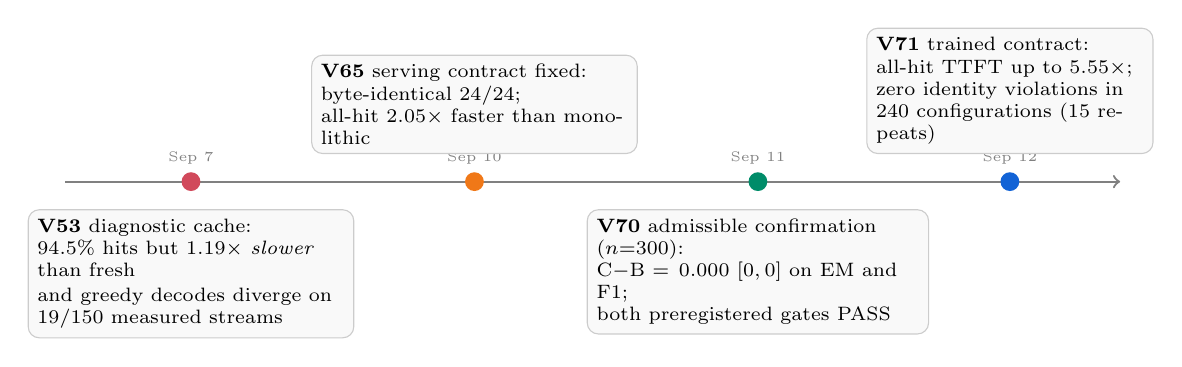
\begin{tikzpicture}[font=\scriptsize]
  \draw[gray, thick, ->] (0,0) -- (13.4,0);
  \node[circle, fill=ddiRed,   inner sep=2.4pt] (v53) at (1.6,0) {};
  \node[circle, fill=ddiGold,  inner sep=2.4pt] (v65) at (5.2,0) {};
  \node[circle, fill=ddiGreen, inner sep=2.4pt] (v70) at (8.8,0) {};
  \node[circle, fill=ddiBlue,  inner sep=2.4pt] (v71) at (12.0,0) {};
  \node[font=\tiny, gray, anchor=south] at (1.6,0.10) {Sep 7};
  \node[font=\tiny, gray, anchor=south] at (5.2,0.10) {Sep 10};
  \node[font=\tiny, gray, anchor=south] at (8.8,0.10) {Sep 11};
  \node[font=\tiny, gray, anchor=south] at (12.0,0.10) {Sep 12};
  \node[draw=gray!40, fill=gray!5, rounded corners, align=left, anchor=north, text width=3.9cm]
    at (1.6,-0.35)
    {\textbf{V53} diagnostic cache:\\ 94.5\% hits but $1.19\times$
     \emph{slower} than fresh\\ [1pt] and greedy decodes diverge on 19/150 measured streams};
  \node[draw=gray!40, fill=gray!5, rounded corners, align=left, anchor=south, text width=3.9cm]
    at (5.2,0.35)
    {\textbf{V65} serving contract fixed:\\ byte-identical 24/24;\\
     all-hit $2.05\times$ faster than monolithic};
  \node[draw=gray!40, fill=gray!5, rounded corners, align=left, anchor=north, text width=4.1cm]
    at (8.8,-0.35)
    {\textbf{V70} admissible confirmation ($n{=}$300$)$:\\
     C$-$B $=0.000$ $[0,0]$ on EM and F1;\\ both preregistered gates PASS};
  \node[draw=gray!40, fill=gray!5, rounded corners, align=left, anchor=south, text width=3.4cm]
    at (12.0,0.35)
    {\textbf{V71} trained contract:\\ all-hit TTFT up to $5.55\times$;\\
     zero identity violations in 240 configurations (15 repeats)};
\end{tikzpicture}

\caption{Program arc from diagnostic cache to production trained
contract. V53: a warm cache that is neither faithful nor fast. V65: the
serving contract made byte-identical and fast. V70/V72: admissible
$n{=}300$ confirmation with an exact-zero identity gate, replicated across
seeds and model families (V72-a/V72-b in Fig.~\ref{fig:gatedeltas}; the
stations reuse the same frozen records). V71: the trained contract keeps
the serving win. All displayed values are rendered from the pinned ledger.}
\label{fig:timeline}
\end{figure}

\paragraph{Prefix-cache baseline, redone genuinely (V112).}
The withdrawn V73 comparison was rebuilt from scratch
(VIBEQUEUE-114; prereg frozen before the run). The new harness implements a
real exact-prefix cache: document-prefix K/V tensors are stored keyed by the
\emph{ordered} document token tuple, and a hit loads them and prefills only
the query tail --- verified by an instrumented counter that shows hits
forward zero document tokens (the positive control the review demanded),
and by a byte-identity gate on the first miss.

\begin{table}[H]
\centering\footnotesize% Generated by paper/render.py from paper/evidence.json.
% Sources: results/v112_prefix_cache_redo_20260917T100727Z/summary.json sha256=e9592e47dfd73827ee7054e25310b202de107f76ab304660e4cead22eadf023b.
\resizebox{\linewidth}{!}{%
\begin{tabular}{lrrr}
\toprule
Arm & prefill ms & TTFT ms & total ms \\
\midrule
monolithic (no cache) & 664.9 & 695.9 & 868.5 \\
prefix cache, fixed order (hits) & 54.3 & 81.9 & 222.4 \\
prefix cache, reordered (all miss) & 665.3 & 694.7 & 839.0 \\
DDI canonical, fixed order (all hit) & --- & --- & 771.2 \\
DDI canonical, reordered (all hit) & --- & --- & 773.3 \\
\midrule
\multicolumn{4}{p{0.97\linewidth}}{\footnotesize Genuine exact-prefix KV cache: hits load stored document-prefix K/V and prefill only the query tail (instrumented); the first miss is byte-identical to monolithic. Prefix keys are ordered document tuples, so reordering misses every time while DDI's content-addressed keys keep their win. Hit outputs match monolithic on 90\% of requests (bf16 reduction-order divergence; measured, not gated) --- DDI's canonical exact identity remains the contrast.} \\
\bottomrule
\end{tabular}}

\caption{Prefix-cache redo (V112): fixed-order traffic, reordered traffic,
and the DDI canonical cache on the same requests.}
\label{tab:prefixredo}
\end{table}

The measured outcome (Table~\ref{tab:prefixredo}): in fixed-order traffic
the prefix cache cuts median prefill from 664.9\,ms to 54.3\,ms
($12.2\times$; TTFT $8.5\times$) --- a real serving win that the broken V73
harness never exercised. Under per-request document reordering its
ordered-tuple keys miss every time and it degrades exactly to monolithic
(665.3 vs 664.9\,ms), while DDI's content-addressed per-document keys keep
their win under both orders. Two honest caveats distinguish this baseline
from the DDI contract: prefix hits reproduce monolithic outputs on 90\% of
requests (bf16 reduction-order divergence between the standalone prefix
forward and the full-stream forward --- measured, not gated), and the cache
is order-dependent by construction. The DDI canonical contract remains the
only path that is simultaneously order-independent \emph{and}
byte-identical.

\section{Coverage and Limits}
\label{sec:coverage}

\begin{figure}[H]
\centering% Generated by paper/render.py; aggregates: paper/evidence.json.
% Sources: VIBEQUEUE-53-REPORT.md sha256=7cd9223e128c5d82b61e59575035fe4bb54c9f48c5da721723fd5d214d85195e; results/cache_v53_local_20260907/summary.json sha256=28ae886d9dae851ed090b7ebb0744b33926060d9499c3f16a01221810a0e2189; results/cache_v53_local_20260907/timing.jsonl sha256=055cf47312269ca147c6d4517d26b82aabc910b11fd6ca07f5eba5e3f54153a8; results/cache_v53_local_20260907/validation.jsonl sha256=8597c0b5394b4b17248065ad1ebc386a0a2d864f089f8e65d51d5e293f7b8d4a; results/phase3_n10.jsonl sha256=1d0a7c012582a0af40c322e6c3b91540e083ee27b2bb5a896cc9230442470dda; results/phase3_n2.jsonl sha256=1c2d4b3068468e1f76249bb1bfdc9f579797fec06f0e45b9cc8e2ef5085407c2; results/phase3_n5.jsonl sha256=6d18b180ae2df48856d304cc1184f4fbf6f76661226cd8e075eee3dea765bd34; results/runs.jsonl sha256=70c098a691f9c485bd8b3ce6a3304749969f3c4d3eb4f812539bdcd867a31b47; results/sprint_c_llama.jsonl sha256=c7edb5045db9479bfcdcf403b3e38daaebf28af6fd48f14b5438000d7695ff02; results/sprint_c_1.5B.jsonl sha256=c52ef34b36b9582c88643a5a61f0ce17a87e036cfe334f23d4887808f8e23cd0; results/sprint_a_strict_base.jsonl sha256=b1196a2c1f3577c3d78b75b22d47dff7e0a14c538d428d4b0a81a1c81fa6f9fc
\begin{tabular}{@{}p{4.3cm}p{5.4cm}p{5.4cm}@{}}
\toprule
\textbf{Requested relationship} & \textbf{Measured (validation program)} &
\textbf{Still missing} \\
\midrule
Quality / prefill speedup & \textcolor{ddiBlue}{V57: matched full-vs-DDI QA + timing, same 100 requests} &
\textcolor{ddiRed}{Matched QA under a validated sparse kernel} \\[5pt]
Quality / KV reuse & \textcolor{ddiGreen}{V58 + V65: gold-answer QA under hits; V64 audited;
V68 divergence anatomy; V70 trained contract: C$-$B exactly zero, $n{=}300$, both gates passed} &
\textcolor{ddiRed}{Multi-seed robustness; scale beyond $n{=}300$} \\[5pt]
Warm-path serving win & \textcolor{ddiGreen}{V65: 2.05$\times$ TTFT, byte-identical, gate passed} &
\textcolor{ddiRed}{Mixed/partial-hit beating baseline; prefix-cache baseline; trained-contract serving latency} \\[5pt]
Hit rate / sparsity & \textcolor{ddiPurple}{V59 measured crossover + analytical surface} &
\textcolor{ddiRed}{Controlled workload$\times$mask sweep at scale} \\
\bottomrule
\end{tabular}

\caption{Evidence coverage. Previously red quality--timing and
quality--reuse joins are measured (V57, V58, V65, V68, V70, V71, V72);
remaining red: mixed/partial-hit schedules beyond crossovers and a
validated sparse-plus-reuse combination.}
\label{fig:coverage}
\end{figure}

\begin{figure}[H]
\centering\resizebox{.88\linewidth}{!}{% Generated by paper/render.py; aggregates: paper/evidence.json.
% Sources: VIBEQUEUE-53-REPORT.md sha256=7cd9223e128c5d82b61e59575035fe4bb54c9f48c5da721723fd5d214d85195e; results/cache_v53_local_20260907/summary.json sha256=28ae886d9dae851ed090b7ebb0744b33926060d9499c3f16a01221810a0e2189; results/cache_v53_local_20260907/timing.jsonl sha256=055cf47312269ca147c6d4517d26b82aabc910b11fd6ca07f5eba5e3f54153a8; results/cache_v53_local_20260907/validation.jsonl sha256=8597c0b5394b4b17248065ad1ebc386a0a2d864f089f8e65d51d5e293f7b8d4a; ddi/masks.py sha256=2ee804f18a94f4bd709b7629d4962a7c47f732157284c4218f31239956ba7f54
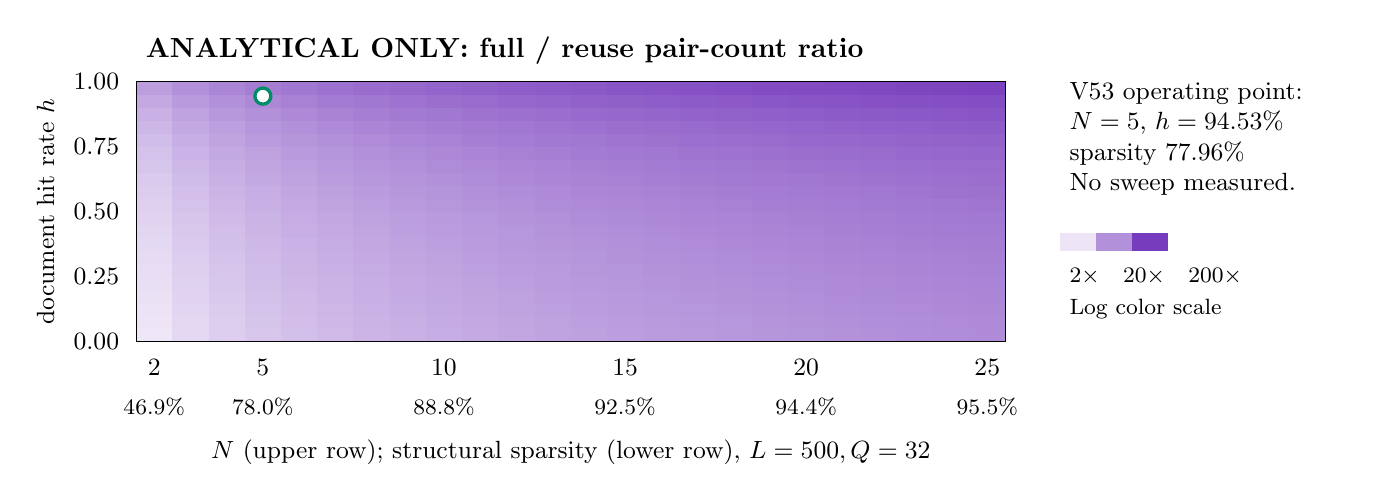
\begin{tikzpicture}[x=.46cm,y=3.3cm,font=\small]
\fill[ddiPurple!12.37!white] (1.5,0.0) rectangle ++(1,.05);
\fill[ddiPurple!13.24!white] (1.5,0.05) rectangle ++(1,.05);
\fill[ddiPurple!14.16!white] (1.5,0.1) rectangle ++(1,.05);
\fill[ddiPurple!15.12!white] (1.5,0.15) rectangle ++(1,.05);
\fill[ddiPurple!16.14!white] (1.5,0.2) rectangle ++(1,.05);
\fill[ddiPurple!17.21!white] (1.5,0.25) rectangle ++(1,.05);
\fill[ddiPurple!18.35!white] (1.5,0.3) rectangle ++(1,.05);
\fill[ddiPurple!19.56!white] (1.5,0.35) rectangle ++(1,.05);
\fill[ddiPurple!20.85!white] (1.5,0.4) rectangle ++(1,.05);
\fill[ddiPurple!22.24!white] (1.5,0.45) rectangle ++(1,.05);
\fill[ddiPurple!23.74!white] (1.5,0.5) rectangle ++(1,.05);
\fill[ddiPurple!25.37!white] (1.5,0.55) rectangle ++(1,.05);
\fill[ddiPurple!27.15!white] (1.5,0.6) rectangle ++(1,.05);
\fill[ddiPurple!29.12!white] (1.5,0.65) rectangle ++(1,.05);
\fill[ddiPurple!31.32!white] (1.5,0.7) rectangle ++(1,.05);
\fill[ddiPurple!33.81!white] (1.5,0.75) rectangle ++(1,.05);
\fill[ddiPurple!36.67!white] (1.5,0.8) rectangle ++(1,.05);
\fill[ddiPurple!40.05!white] (1.5,0.85) rectangle ++(1,.05);
\fill[ddiPurple!44.18!white] (1.5,0.9) rectangle ++(1,.05);
\fill[ddiPurple!49.46!white] (1.5,0.95) rectangle ++(1,.05);
\fill[ddiPurple!19.64!white] (2.5,0.0) rectangle ++(1,.05);
\fill[ddiPurple!20.51!white] (2.5,0.05) rectangle ++(1,.05);
\fill[ddiPurple!21.43!white] (2.5,0.1) rectangle ++(1,.05);
\fill[ddiPurple!22.39!white] (2.5,0.15) rectangle ++(1,.05);
\fill[ddiPurple!23.41!white] (2.5,0.2) rectangle ++(1,.05);
\fill[ddiPurple!24.48!white] (2.5,0.25) rectangle ++(1,.05);
\fill[ddiPurple!25.62!white] (2.5,0.3) rectangle ++(1,.05);
\fill[ddiPurple!26.83!white] (2.5,0.35) rectangle ++(1,.05);
\fill[ddiPurple!28.13!white] (2.5,0.4) rectangle ++(1,.05);
\fill[ddiPurple!29.52!white] (2.5,0.45) rectangle ++(1,.05);
\fill[ddiPurple!31.02!white] (2.5,0.5) rectangle ++(1,.05);
\fill[ddiPurple!32.65!white] (2.5,0.55) rectangle ++(1,.05);
\fill[ddiPurple!34.43!white] (2.5,0.6) rectangle ++(1,.05);
\fill[ddiPurple!36.40!white] (2.5,0.65) rectangle ++(1,.05);
\fill[ddiPurple!38.61!white] (2.5,0.7) rectangle ++(1,.05);
\fill[ddiPurple!41.10!white] (2.5,0.75) rectangle ++(1,.05);
\fill[ddiPurple!43.97!white] (2.5,0.8) rectangle ++(1,.05);
\fill[ddiPurple!47.36!white] (2.5,0.85) rectangle ++(1,.05);
\fill[ddiPurple!51.50!white] (2.5,0.9) rectangle ++(1,.05);
\fill[ddiPurple!56.80!white] (2.5,0.95) rectangle ++(1,.05);
\fill[ddiPurple!24.87!white] (3.5,0.0) rectangle ++(1,.05);
\fill[ddiPurple!25.75!white] (3.5,0.05) rectangle ++(1,.05);
\fill[ddiPurple!26.66!white] (3.5,0.1) rectangle ++(1,.05);
\fill[ddiPurple!27.63!white] (3.5,0.15) rectangle ++(1,.05);
\fill[ddiPurple!28.64!white] (3.5,0.2) rectangle ++(1,.05);
\fill[ddiPurple!29.72!white] (3.5,0.25) rectangle ++(1,.05);
\fill[ddiPurple!30.86!white] (3.5,0.3) rectangle ++(1,.05);
\fill[ddiPurple!32.07!white] (3.5,0.35) rectangle ++(1,.05);
\fill[ddiPurple!33.37!white] (3.5,0.4) rectangle ++(1,.05);
\fill[ddiPurple!34.76!white] (3.5,0.45) rectangle ++(1,.05);
\fill[ddiPurple!36.26!white] (3.5,0.5) rectangle ++(1,.05);
\fill[ddiPurple!37.89!white] (3.5,0.55) rectangle ++(1,.05);
\fill[ddiPurple!39.68!white] (3.5,0.6) rectangle ++(1,.05);
\fill[ddiPurple!41.65!white] (3.5,0.65) rectangle ++(1,.05);
\fill[ddiPurple!43.85!white] (3.5,0.7) rectangle ++(1,.05);
\fill[ddiPurple!46.35!white] (3.5,0.75) rectangle ++(1,.05);
\fill[ddiPurple!49.22!white] (3.5,0.8) rectangle ++(1,.05);
\fill[ddiPurple!52.62!white] (3.5,0.85) rectangle ++(1,.05);
\fill[ddiPurple!56.76!white] (3.5,0.9) rectangle ++(1,.05);
\fill[ddiPurple!62.07!white] (3.5,0.95) rectangle ++(1,.05);
\fill[ddiPurple!28.97!white] (4.5,0.0) rectangle ++(1,.05);
\fill[ddiPurple!29.84!white] (4.5,0.05) rectangle ++(1,.05);
\fill[ddiPurple!30.76!white] (4.5,0.1) rectangle ++(1,.05);
\fill[ddiPurple!31.72!white] (4.5,0.15) rectangle ++(1,.05);
\fill[ddiPurple!32.74!white] (4.5,0.2) rectangle ++(1,.05);
\fill[ddiPurple!33.81!white] (4.5,0.25) rectangle ++(1,.05);
\fill[ddiPurple!34.95!white] (4.5,0.3) rectangle ++(1,.05);
\fill[ddiPurple!36.17!white] (4.5,0.35) rectangle ++(1,.05);
\fill[ddiPurple!37.46!white] (4.5,0.4) rectangle ++(1,.05);
\fill[ddiPurple!38.85!white] (4.5,0.45) rectangle ++(1,.05);
\fill[ddiPurple!40.36!white] (4.5,0.5) rectangle ++(1,.05);
\fill[ddiPurple!41.99!white] (4.5,0.55) rectangle ++(1,.05);
\fill[ddiPurple!43.77!white] (4.5,0.6) rectangle ++(1,.05);
\fill[ddiPurple!45.75!white] (4.5,0.65) rectangle ++(1,.05);
\fill[ddiPurple!47.95!white] (4.5,0.7) rectangle ++(1,.05);
\fill[ddiPurple!50.45!white] (4.5,0.75) rectangle ++(1,.05);
\fill[ddiPurple!53.33!white] (4.5,0.8) rectangle ++(1,.05);
\fill[ddiPurple!56.72!white] (4.5,0.85) rectangle ++(1,.05);
\fill[ddiPurple!60.87!white] (4.5,0.9) rectangle ++(1,.05);
\fill[ddiPurple!66.19!white] (4.5,0.95) rectangle ++(1,.05);
\fill[ddiPurple!32.33!white] (5.5,0.0) rectangle ++(1,.05);
\fill[ddiPurple!33.20!white] (5.5,0.05) rectangle ++(1,.05);
\fill[ddiPurple!34.12!white] (5.5,0.1) rectangle ++(1,.05);
\fill[ddiPurple!35.09!white] (5.5,0.15) rectangle ++(1,.05);
\fill[ddiPurple!36.10!white] (5.5,0.2) rectangle ++(1,.05);
\fill[ddiPurple!37.18!white] (5.5,0.25) rectangle ++(1,.05);
\fill[ddiPurple!38.32!white] (5.5,0.3) rectangle ++(1,.05);
\fill[ddiPurple!39.53!white] (5.5,0.35) rectangle ++(1,.05);
\fill[ddiPurple!40.83!white] (5.5,0.4) rectangle ++(1,.05);
\fill[ddiPurple!42.22!white] (5.5,0.45) rectangle ++(1,.05);
\fill[ddiPurple!43.72!white] (5.5,0.5) rectangle ++(1,.05);
\fill[ddiPurple!45.35!white] (5.5,0.55) rectangle ++(1,.05);
\fill[ddiPurple!47.14!white] (5.5,0.6) rectangle ++(1,.05);
\fill[ddiPurple!49.11!white] (5.5,0.65) rectangle ++(1,.05);
\fill[ddiPurple!51.32!white] (5.5,0.7) rectangle ++(1,.05);
\fill[ddiPurple!53.82!white] (5.5,0.75) rectangle ++(1,.05);
\fill[ddiPurple!56.69!white] (5.5,0.8) rectangle ++(1,.05);
\fill[ddiPurple!60.09!white] (5.5,0.85) rectangle ++(1,.05);
\fill[ddiPurple!64.24!white] (5.5,0.9) rectangle ++(1,.05);
\fill[ddiPurple!69.56!white] (5.5,0.95) rectangle ++(1,.05);
\fill[ddiPurple!35.18!white] (6.5,0.0) rectangle ++(1,.05);
\fill[ddiPurple!36.06!white] (6.5,0.05) rectangle ++(1,.05);
\fill[ddiPurple!36.98!white] (6.5,0.1) rectangle ++(1,.05);
\fill[ddiPurple!37.94!white] (6.5,0.15) rectangle ++(1,.05);
\fill[ddiPurple!38.96!white] (6.5,0.2) rectangle ++(1,.05);
\fill[ddiPurple!40.03!white] (6.5,0.25) rectangle ++(1,.05);
\fill[ddiPurple!41.17!white] (6.5,0.3) rectangle ++(1,.05);
\fill[ddiPurple!42.38!white] (6.5,0.35) rectangle ++(1,.05);
\fill[ddiPurple!43.68!white] (6.5,0.4) rectangle ++(1,.05);
\fill[ddiPurple!45.07!white] (6.5,0.45) rectangle ++(1,.05);
\fill[ddiPurple!46.57!white] (6.5,0.5) rectangle ++(1,.05);
\fill[ddiPurple!48.21!white] (6.5,0.55) rectangle ++(1,.05);
\fill[ddiPurple!49.99!white] (6.5,0.6) rectangle ++(1,.05);
\fill[ddiPurple!51.97!white] (6.5,0.65) rectangle ++(1,.05);
\fill[ddiPurple!54.17!white] (6.5,0.7) rectangle ++(1,.05);
\fill[ddiPurple!56.67!white] (6.5,0.75) rectangle ++(1,.05);
\fill[ddiPurple!59.55!white] (6.5,0.8) rectangle ++(1,.05);
\fill[ddiPurple!62.95!white] (6.5,0.85) rectangle ++(1,.05);
\fill[ddiPurple!67.10!white] (6.5,0.9) rectangle ++(1,.05);
\fill[ddiPurple!72.43!white] (6.5,0.95) rectangle ++(1,.05);
\fill[ddiPurple!37.66!white] (7.5,0.0) rectangle ++(1,.05);
\fill[ddiPurple!38.54!white] (7.5,0.05) rectangle ++(1,.05);
\fill[ddiPurple!39.45!white] (7.5,0.1) rectangle ++(1,.05);
\fill[ddiPurple!40.42!white] (7.5,0.15) rectangle ++(1,.05);
\fill[ddiPurple!41.44!white] (7.5,0.2) rectangle ++(1,.05);
\fill[ddiPurple!42.51!white] (7.5,0.25) rectangle ++(1,.05);
\fill[ddiPurple!43.65!white] (7.5,0.3) rectangle ++(1,.05);
\fill[ddiPurple!44.86!white] (7.5,0.35) rectangle ++(1,.05);
\fill[ddiPurple!46.16!white] (7.5,0.4) rectangle ++(1,.05);
\fill[ddiPurple!47.55!white] (7.5,0.45) rectangle ++(1,.05);
\fill[ddiPurple!49.05!white] (7.5,0.5) rectangle ++(1,.05);
\fill[ddiPurple!50.69!white] (7.5,0.55) rectangle ++(1,.05);
\fill[ddiPurple!52.47!white] (7.5,0.6) rectangle ++(1,.05);
\fill[ddiPurple!54.45!white] (7.5,0.65) rectangle ++(1,.05);
\fill[ddiPurple!56.66!white] (7.5,0.7) rectangle ++(1,.05);
\fill[ddiPurple!59.15!white] (7.5,0.75) rectangle ++(1,.05);
\fill[ddiPurple!62.03!white] (7.5,0.8) rectangle ++(1,.05);
\fill[ddiPurple!65.43!white] (7.5,0.85) rectangle ++(1,.05);
\fill[ddiPurple!69.59!white] (7.5,0.9) rectangle ++(1,.05);
\fill[ddiPurple!74.91!white] (7.5,0.95) rectangle ++(1,.05);
\fill[ddiPurple!39.85!white] (8.5,0.0) rectangle ++(1,.05);
\fill[ddiPurple!40.73!white] (8.5,0.05) rectangle ++(1,.05);
\fill[ddiPurple!41.64!white] (8.5,0.1) rectangle ++(1,.05);
\fill[ddiPurple!42.61!white] (8.5,0.15) rectangle ++(1,.05);
\fill[ddiPurple!43.63!white] (8.5,0.2) rectangle ++(1,.05);
\fill[ddiPurple!44.70!white] (8.5,0.25) rectangle ++(1,.05);
\fill[ddiPurple!45.84!white] (8.5,0.3) rectangle ++(1,.05);
\fill[ddiPurple!47.05!white] (8.5,0.35) rectangle ++(1,.05);
\fill[ddiPurple!48.35!white] (8.5,0.4) rectangle ++(1,.05);
\fill[ddiPurple!49.74!white] (8.5,0.45) rectangle ++(1,.05);
\fill[ddiPurple!51.24!white] (8.5,0.5) rectangle ++(1,.05);
\fill[ddiPurple!52.88!white] (8.5,0.55) rectangle ++(1,.05);
\fill[ddiPurple!54.67!white] (8.5,0.6) rectangle ++(1,.05);
\fill[ddiPurple!56.64!white] (8.5,0.65) rectangle ++(1,.05);
\fill[ddiPurple!58.85!white] (8.5,0.7) rectangle ++(1,.05);
\fill[ddiPurple!61.35!white] (8.5,0.75) rectangle ++(1,.05);
\fill[ddiPurple!64.23!white] (8.5,0.8) rectangle ++(1,.05);
\fill[ddiPurple!67.63!white] (8.5,0.85) rectangle ++(1,.05);
\fill[ddiPurple!71.78!white] (8.5,0.9) rectangle ++(1,.05);
\fill[ddiPurple!77.11!white] (8.5,0.95) rectangle ++(1,.05);
\fill[ddiPurple!41.81!white] (9.5,0.0) rectangle ++(1,.05);
\fill[ddiPurple!42.69!white] (9.5,0.05) rectangle ++(1,.05);
\fill[ddiPurple!43.61!white] (9.5,0.1) rectangle ++(1,.05);
\fill[ddiPurple!44.57!white] (9.5,0.15) rectangle ++(1,.05);
\fill[ddiPurple!45.59!white] (9.5,0.2) rectangle ++(1,.05);
\fill[ddiPurple!46.66!white] (9.5,0.25) rectangle ++(1,.05);
\fill[ddiPurple!47.80!white] (9.5,0.3) rectangle ++(1,.05);
\fill[ddiPurple!49.02!white] (9.5,0.35) rectangle ++(1,.05);
\fill[ddiPurple!50.31!white] (9.5,0.4) rectangle ++(1,.05);
\fill[ddiPurple!51.70!white] (9.5,0.45) rectangle ++(1,.05);
\fill[ddiPurple!53.21!white] (9.5,0.5) rectangle ++(1,.05);
\fill[ddiPurple!54.84!white] (9.5,0.55) rectangle ++(1,.05);
\fill[ddiPurple!56.63!white] (9.5,0.6) rectangle ++(1,.05);
\fill[ddiPurple!58.60!white] (9.5,0.65) rectangle ++(1,.05);
\fill[ddiPurple!60.81!white] (9.5,0.7) rectangle ++(1,.05);
\fill[ddiPurple!63.31!white] (9.5,0.75) rectangle ++(1,.05);
\fill[ddiPurple!66.19!white] (9.5,0.8) rectangle ++(1,.05);
\fill[ddiPurple!69.59!white] (9.5,0.85) rectangle ++(1,.05);
\fill[ddiPurple!73.75!white] (9.5,0.9) rectangle ++(1,.05);
\fill[ddiPurple!79.08!white] (9.5,0.95) rectangle ++(1,.05);
\fill[ddiPurple!43.59!white] (10.5,0.0) rectangle ++(1,.05);
\fill[ddiPurple!44.47!white] (10.5,0.05) rectangle ++(1,.05);
\fill[ddiPurple!45.38!white] (10.5,0.1) rectangle ++(1,.05);
\fill[ddiPurple!46.35!white] (10.5,0.15) rectangle ++(1,.05);
\fill[ddiPurple!47.37!white] (10.5,0.2) rectangle ++(1,.05);
\fill[ddiPurple!48.44!white] (10.5,0.25) rectangle ++(1,.05);
\fill[ddiPurple!49.58!white] (10.5,0.3) rectangle ++(1,.05);
\fill[ddiPurple!50.79!white] (10.5,0.35) rectangle ++(1,.05);
\fill[ddiPurple!52.09!white] (10.5,0.4) rectangle ++(1,.05);
\fill[ddiPurple!53.48!white] (10.5,0.45) rectangle ++(1,.05);
\fill[ddiPurple!54.99!white] (10.5,0.5) rectangle ++(1,.05);
\fill[ddiPurple!56.62!white] (10.5,0.55) rectangle ++(1,.05);
\fill[ddiPurple!58.41!white] (10.5,0.6) rectangle ++(1,.05);
\fill[ddiPurple!60.38!white] (10.5,0.65) rectangle ++(1,.05);
\fill[ddiPurple!62.59!white] (10.5,0.7) rectangle ++(1,.05);
\fill[ddiPurple!65.09!white] (10.5,0.75) rectangle ++(1,.05);
\fill[ddiPurple!67.97!white] (10.5,0.8) rectangle ++(1,.05);
\fill[ddiPurple!71.37!white] (10.5,0.85) rectangle ++(1,.05);
\fill[ddiPurple!75.53!white] (10.5,0.9) rectangle ++(1,.05);
\fill[ddiPurple!80.86!white] (10.5,0.95) rectangle ++(1,.05);
\fill[ddiPurple!45.21!white] (11.5,0.0) rectangle ++(1,.05);
\fill[ddiPurple!46.09!white] (11.5,0.05) rectangle ++(1,.05);
\fill[ddiPurple!47.01!white] (11.5,0.1) rectangle ++(1,.05);
\fill[ddiPurple!47.97!white] (11.5,0.15) rectangle ++(1,.05);
\fill[ddiPurple!48.99!white] (11.5,0.2) rectangle ++(1,.05);
\fill[ddiPurple!50.06!white] (11.5,0.25) rectangle ++(1,.05);
\fill[ddiPurple!51.20!white] (11.5,0.3) rectangle ++(1,.05);
\fill[ddiPurple!52.42!white] (11.5,0.35) rectangle ++(1,.05);
\fill[ddiPurple!53.71!white] (11.5,0.4) rectangle ++(1,.05);
\fill[ddiPurple!55.11!white] (11.5,0.45) rectangle ++(1,.05);
\fill[ddiPurple!56.61!white] (11.5,0.5) rectangle ++(1,.05);
\fill[ddiPurple!58.24!white] (11.5,0.55) rectangle ++(1,.05);
\fill[ddiPurple!60.03!white] (11.5,0.6) rectangle ++(1,.05);
\fill[ddiPurple!62.01!white] (11.5,0.65) rectangle ++(1,.05);
\fill[ddiPurple!64.21!white] (11.5,0.7) rectangle ++(1,.05);
\fill[ddiPurple!66.71!white] (11.5,0.75) rectangle ++(1,.05);
\fill[ddiPurple!69.60!white] (11.5,0.8) rectangle ++(1,.05);
\fill[ddiPurple!73.00!white] (11.5,0.85) rectangle ++(1,.05);
\fill[ddiPurple!77.15!white] (11.5,0.9) rectangle ++(1,.05);
\fill[ddiPurple!82.49!white] (11.5,0.95) rectangle ++(1,.05);
\fill[ddiPurple!46.71!white] (12.5,0.0) rectangle ++(1,.05);
\fill[ddiPurple!47.59!white] (12.5,0.05) rectangle ++(1,.05);
\fill[ddiPurple!48.50!white] (12.5,0.1) rectangle ++(1,.05);
\fill[ddiPurple!49.47!white] (12.5,0.15) rectangle ++(1,.05);
\fill[ddiPurple!50.49!white] (12.5,0.2) rectangle ++(1,.05);
\fill[ddiPurple!51.56!white] (12.5,0.25) rectangle ++(1,.05);
\fill[ddiPurple!52.70!white] (12.5,0.3) rectangle ++(1,.05);
\fill[ddiPurple!53.91!white] (12.5,0.35) rectangle ++(1,.05);
\fill[ddiPurple!55.21!white] (12.5,0.4) rectangle ++(1,.05);
\fill[ddiPurple!56.60!white] (12.5,0.45) rectangle ++(1,.05);
\fill[ddiPurple!58.11!white] (12.5,0.5) rectangle ++(1,.05);
\fill[ddiPurple!59.74!white] (12.5,0.55) rectangle ++(1,.05);
\fill[ddiPurple!61.53!white] (12.5,0.6) rectangle ++(1,.05);
\fill[ddiPurple!63.50!white] (12.5,0.65) rectangle ++(1,.05);
\fill[ddiPurple!65.71!white] (12.5,0.7) rectangle ++(1,.05);
\fill[ddiPurple!68.21!white] (12.5,0.75) rectangle ++(1,.05);
\fill[ddiPurple!71.09!white] (12.5,0.8) rectangle ++(1,.05);
\fill[ddiPurple!74.50!white] (12.5,0.85) rectangle ++(1,.05);
\fill[ddiPurple!78.65!white] (12.5,0.9) rectangle ++(1,.05);
\fill[ddiPurple!83.99!white] (12.5,0.95) rectangle ++(1,.05);
\fill[ddiPurple!48.10!white] (13.5,0.0) rectangle ++(1,.05);
\fill[ddiPurple!48.97!white] (13.5,0.05) rectangle ++(1,.05);
\fill[ddiPurple!49.89!white] (13.5,0.1) rectangle ++(1,.05);
\fill[ddiPurple!50.85!white] (13.5,0.15) rectangle ++(1,.05);
\fill[ddiPurple!51.87!white] (13.5,0.2) rectangle ++(1,.05);
\fill[ddiPurple!52.95!white] (13.5,0.25) rectangle ++(1,.05);
\fill[ddiPurple!54.09!white] (13.5,0.3) rectangle ++(1,.05);
\fill[ddiPurple!55.30!white] (13.5,0.35) rectangle ++(1,.05);
\fill[ddiPurple!56.60!white] (13.5,0.4) rectangle ++(1,.05);
\fill[ddiPurple!57.99!white] (13.5,0.45) rectangle ++(1,.05);
\fill[ddiPurple!59.49!white] (13.5,0.5) rectangle ++(1,.05);
\fill[ddiPurple!61.13!white] (13.5,0.55) rectangle ++(1,.05);
\fill[ddiPurple!62.91!white] (13.5,0.6) rectangle ++(1,.05);
\fill[ddiPurple!64.89!white] (13.5,0.65) rectangle ++(1,.05);
\fill[ddiPurple!67.10!white] (13.5,0.7) rectangle ++(1,.05);
\fill[ddiPurple!69.60!white] (13.5,0.75) rectangle ++(1,.05);
\fill[ddiPurple!72.48!white] (13.5,0.8) rectangle ++(1,.05);
\fill[ddiPurple!75.88!white] (13.5,0.85) rectangle ++(1,.05);
\fill[ddiPurple!80.04!white] (13.5,0.9) rectangle ++(1,.05);
\fill[ddiPurple!85.37!white] (13.5,0.95) rectangle ++(1,.05);
\fill[ddiPurple!49.39!white] (14.5,0.0) rectangle ++(1,.05);
\fill[ddiPurple!50.26!white] (14.5,0.05) rectangle ++(1,.05);
\fill[ddiPurple!51.18!white] (14.5,0.1) rectangle ++(1,.05);
\fill[ddiPurple!52.15!white] (14.5,0.15) rectangle ++(1,.05);
\fill[ddiPurple!53.16!white] (14.5,0.2) rectangle ++(1,.05);
\fill[ddiPurple!54.24!white] (14.5,0.25) rectangle ++(1,.05);
\fill[ddiPurple!55.38!white] (14.5,0.3) rectangle ++(1,.05);
\fill[ddiPurple!56.59!white] (14.5,0.35) rectangle ++(1,.05);
\fill[ddiPurple!57.89!white] (14.5,0.4) rectangle ++(1,.05);
\fill[ddiPurple!59.28!white] (14.5,0.45) rectangle ++(1,.05);
\fill[ddiPurple!60.78!white] (14.5,0.5) rectangle ++(1,.05);
\fill[ddiPurple!62.42!white] (14.5,0.55) rectangle ++(1,.05);
\fill[ddiPurple!64.21!white] (14.5,0.6) rectangle ++(1,.05);
\fill[ddiPurple!66.18!white] (14.5,0.65) rectangle ++(1,.05);
\fill[ddiPurple!68.39!white] (14.5,0.7) rectangle ++(1,.05);
\fill[ddiPurple!70.89!white] (14.5,0.75) rectangle ++(1,.05);
\fill[ddiPurple!73.77!white] (14.5,0.8) rectangle ++(1,.05);
\fill[ddiPurple!77.17!white] (14.5,0.85) rectangle ++(1,.05);
\fill[ddiPurple!81.33!white] (14.5,0.9) rectangle ++(1,.05);
\fill[ddiPurple!86.67!white] (14.5,0.95) rectangle ++(1,.05);
\fill[ddiPurple!50.59!white] (15.5,0.0) rectangle ++(1,.05);
\fill[ddiPurple!51.47!white] (15.5,0.05) rectangle ++(1,.05);
\fill[ddiPurple!52.39!white] (15.5,0.1) rectangle ++(1,.05);
\fill[ddiPurple!53.35!white] (15.5,0.15) rectangle ++(1,.05);
\fill[ddiPurple!54.37!white] (15.5,0.2) rectangle ++(1,.05);
\fill[ddiPurple!55.45!white] (15.5,0.25) rectangle ++(1,.05);
\fill[ddiPurple!56.59!white] (15.5,0.3) rectangle ++(1,.05);
\fill[ddiPurple!57.80!white] (15.5,0.35) rectangle ++(1,.05);
\fill[ddiPurple!59.10!white] (15.5,0.4) rectangle ++(1,.05);
\fill[ddiPurple!60.49!white] (15.5,0.45) rectangle ++(1,.05);
\fill[ddiPurple!61.99!white] (15.5,0.5) rectangle ++(1,.05);
\fill[ddiPurple!63.63!white] (15.5,0.55) rectangle ++(1,.05);
\fill[ddiPurple!65.41!white] (15.5,0.6) rectangle ++(1,.05);
\fill[ddiPurple!67.39!white] (15.5,0.65) rectangle ++(1,.05);
\fill[ddiPurple!69.60!white] (15.5,0.7) rectangle ++(1,.05);
\fill[ddiPurple!72.10!white] (15.5,0.75) rectangle ++(1,.05);
\fill[ddiPurple!74.98!white] (15.5,0.8) rectangle ++(1,.05);
\fill[ddiPurple!78.38!white] (15.5,0.85) rectangle ++(1,.05);
\fill[ddiPurple!82.54!white] (15.5,0.9) rectangle ++(1,.05);
\fill[ddiPurple!87.88!white] (15.5,0.95) rectangle ++(1,.05);
\fill[ddiPurple!51.73!white] (16.5,0.0) rectangle ++(1,.05);
\fill[ddiPurple!52.61!white] (16.5,0.05) rectangle ++(1,.05);
\fill[ddiPurple!53.52!white] (16.5,0.1) rectangle ++(1,.05);
\fill[ddiPurple!54.49!white] (16.5,0.15) rectangle ++(1,.05);
\fill[ddiPurple!55.51!white] (16.5,0.2) rectangle ++(1,.05);
\fill[ddiPurple!56.58!white] (16.5,0.25) rectangle ++(1,.05);
\fill[ddiPurple!57.72!white] (16.5,0.3) rectangle ++(1,.05);
\fill[ddiPurple!58.93!white] (16.5,0.35) rectangle ++(1,.05);
\fill[ddiPurple!60.23!white] (16.5,0.4) rectangle ++(1,.05);
\fill[ddiPurple!61.62!white] (16.5,0.45) rectangle ++(1,.05);
\fill[ddiPurple!63.13!white] (16.5,0.5) rectangle ++(1,.05);
\fill[ddiPurple!64.76!white] (16.5,0.55) rectangle ++(1,.05);
\fill[ddiPurple!66.55!white] (16.5,0.6) rectangle ++(1,.05);
\fill[ddiPurple!68.53!white] (16.5,0.65) rectangle ++(1,.05);
\fill[ddiPurple!70.73!white] (16.5,0.7) rectangle ++(1,.05);
\fill[ddiPurple!73.23!white] (16.5,0.75) rectangle ++(1,.05);
\fill[ddiPurple!76.12!white] (16.5,0.8) rectangle ++(1,.05);
\fill[ddiPurple!79.52!white] (16.5,0.85) rectangle ++(1,.05);
\fill[ddiPurple!83.68!white] (16.5,0.9) rectangle ++(1,.05);
\fill[ddiPurple!89.01!white] (16.5,0.95) rectangle ++(1,.05);
\fill[ddiPurple!52.80!white] (17.5,0.0) rectangle ++(1,.05);
\fill[ddiPurple!53.68!white] (17.5,0.05) rectangle ++(1,.05);
\fill[ddiPurple!54.59!white] (17.5,0.1) rectangle ++(1,.05);
\fill[ddiPurple!55.56!white] (17.5,0.15) rectangle ++(1,.05);
\fill[ddiPurple!56.58!white] (17.5,0.2) rectangle ++(1,.05);
\fill[ddiPurple!57.65!white] (17.5,0.25) rectangle ++(1,.05);
\fill[ddiPurple!58.79!white] (17.5,0.3) rectangle ++(1,.05);
\fill[ddiPurple!60.01!white] (17.5,0.35) rectangle ++(1,.05);
\fill[ddiPurple!61.30!white] (17.5,0.4) rectangle ++(1,.05);
\fill[ddiPurple!62.70!white] (17.5,0.45) rectangle ++(1,.05);
\fill[ddiPurple!64.20!white] (17.5,0.5) rectangle ++(1,.05);
\fill[ddiPurple!65.83!white] (17.5,0.55) rectangle ++(1,.05);
\fill[ddiPurple!67.62!white] (17.5,0.6) rectangle ++(1,.05);
\fill[ddiPurple!69.60!white] (17.5,0.65) rectangle ++(1,.05);
\fill[ddiPurple!71.80!white] (17.5,0.7) rectangle ++(1,.05);
\fill[ddiPurple!74.31!white] (17.5,0.75) rectangle ++(1,.05);
\fill[ddiPurple!77.19!white] (17.5,0.8) rectangle ++(1,.05);
\fill[ddiPurple!80.59!white] (17.5,0.85) rectangle ++(1,.05);
\fill[ddiPurple!84.75!white] (17.5,0.9) rectangle ++(1,.05);
\fill[ddiPurple!90.09!white] (17.5,0.95) rectangle ++(1,.05);
\fill[ddiPurple!53.81!white] (18.5,0.0) rectangle ++(1,.05);
\fill[ddiPurple!54.69!white] (18.5,0.05) rectangle ++(1,.05);
\fill[ddiPurple!55.61!white] (18.5,0.1) rectangle ++(1,.05);
\fill[ddiPurple!56.57!white] (18.5,0.15) rectangle ++(1,.05);
\fill[ddiPurple!57.59!white] (18.5,0.2) rectangle ++(1,.05);
\fill[ddiPurple!58.67!white] (18.5,0.25) rectangle ++(1,.05);
\fill[ddiPurple!59.81!white] (18.5,0.3) rectangle ++(1,.05);
\fill[ddiPurple!61.02!white] (18.5,0.35) rectangle ++(1,.05);
\fill[ddiPurple!62.32!white] (18.5,0.4) rectangle ++(1,.05);
\fill[ddiPurple!63.71!white] (18.5,0.45) rectangle ++(1,.05);
\fill[ddiPurple!65.21!white] (18.5,0.5) rectangle ++(1,.05);
\fill[ddiPurple!66.85!white] (18.5,0.55) rectangle ++(1,.05);
\fill[ddiPurple!68.64!white] (18.5,0.6) rectangle ++(1,.05);
\fill[ddiPurple!70.61!white] (18.5,0.65) rectangle ++(1,.05);
\fill[ddiPurple!72.82!white] (18.5,0.7) rectangle ++(1,.05);
\fill[ddiPurple!75.32!white] (18.5,0.75) rectangle ++(1,.05);
\fill[ddiPurple!78.20!white] (18.5,0.8) rectangle ++(1,.05);
\fill[ddiPurple!81.61!white] (18.5,0.85) rectangle ++(1,.05);
\fill[ddiPurple!85.76!white] (18.5,0.9) rectangle ++(1,.05);
\fill[ddiPurple!91.10!white] (18.5,0.95) rectangle ++(1,.05);
\fill[ddiPurple!54.78!white] (19.5,0.0) rectangle ++(1,.05);
\fill[ddiPurple!55.65!white] (19.5,0.05) rectangle ++(1,.05);
\fill[ddiPurple!56.57!white] (19.5,0.1) rectangle ++(1,.05);
\fill[ddiPurple!57.54!white] (19.5,0.15) rectangle ++(1,.05);
\fill[ddiPurple!58.55!white] (19.5,0.2) rectangle ++(1,.05);
\fill[ddiPurple!59.63!white] (19.5,0.25) rectangle ++(1,.05);
\fill[ddiPurple!60.77!white] (19.5,0.3) rectangle ++(1,.05);
\fill[ddiPurple!61.98!white] (19.5,0.35) rectangle ++(1,.05);
\fill[ddiPurple!63.28!white] (19.5,0.4) rectangle ++(1,.05);
\fill[ddiPurple!64.67!white] (19.5,0.45) rectangle ++(1,.05);
\fill[ddiPurple!66.17!white] (19.5,0.5) rectangle ++(1,.05);
\fill[ddiPurple!67.81!white] (19.5,0.55) rectangle ++(1,.05);
\fill[ddiPurple!69.60!white] (19.5,0.6) rectangle ++(1,.05);
\fill[ddiPurple!71.57!white] (19.5,0.65) rectangle ++(1,.05);
\fill[ddiPurple!73.78!white] (19.5,0.7) rectangle ++(1,.05);
\fill[ddiPurple!76.28!white] (19.5,0.75) rectangle ++(1,.05);
\fill[ddiPurple!79.16!white] (19.5,0.8) rectangle ++(1,.05);
\fill[ddiPurple!82.57!white] (19.5,0.85) rectangle ++(1,.05);
\fill[ddiPurple!86.73!white] (19.5,0.9) rectangle ++(1,.05);
\fill[ddiPurple!92.06!white] (19.5,0.95) rectangle ++(1,.05);
\fill[ddiPurple!55.69!white] (20.5,0.0) rectangle ++(1,.05);
\fill[ddiPurple!56.57!white] (20.5,0.05) rectangle ++(1,.05);
\fill[ddiPurple!57.49!white] (20.5,0.1) rectangle ++(1,.05);
\fill[ddiPurple!58.45!white] (20.5,0.15) rectangle ++(1,.05);
\fill[ddiPurple!59.47!white] (20.5,0.2) rectangle ++(1,.05);
\fill[ddiPurple!60.54!white] (20.5,0.25) rectangle ++(1,.05);
\fill[ddiPurple!61.68!white] (20.5,0.3) rectangle ++(1,.05);
\fill[ddiPurple!62.90!white] (20.5,0.35) rectangle ++(1,.05);
\fill[ddiPurple!64.19!white] (20.5,0.4) rectangle ++(1,.05);
\fill[ddiPurple!65.59!white] (20.5,0.45) rectangle ++(1,.05);
\fill[ddiPurple!67.09!white] (20.5,0.5) rectangle ++(1,.05);
\fill[ddiPurple!68.72!white] (20.5,0.55) rectangle ++(1,.05);
\fill[ddiPurple!70.51!white] (20.5,0.6) rectangle ++(1,.05);
\fill[ddiPurple!72.49!white] (20.5,0.65) rectangle ++(1,.05);
\fill[ddiPurple!74.70!white] (20.5,0.7) rectangle ++(1,.05);
\fill[ddiPurple!77.20!white] (20.5,0.75) rectangle ++(1,.05);
\fill[ddiPurple!80.08!white] (20.5,0.8) rectangle ++(1,.05);
\fill[ddiPurple!83.48!white] (20.5,0.85) rectangle ++(1,.05);
\fill[ddiPurple!87.64!white] (20.5,0.9) rectangle ++(1,.05);
\fill[ddiPurple!92.98!white] (20.5,0.95) rectangle ++(1,.05);
\fill[ddiPurple!56.56!white] (21.5,0.0) rectangle ++(1,.05);
\fill[ddiPurple!57.44!white] (21.5,0.05) rectangle ++(1,.05);
\fill[ddiPurple!58.36!white] (21.5,0.1) rectangle ++(1,.05);
\fill[ddiPurple!59.32!white] (21.5,0.15) rectangle ++(1,.05);
\fill[ddiPurple!60.34!white] (21.5,0.2) rectangle ++(1,.05);
\fill[ddiPurple!61.42!white] (21.5,0.25) rectangle ++(1,.05);
\fill[ddiPurple!62.56!white] (21.5,0.3) rectangle ++(1,.05);
\fill[ddiPurple!63.77!white] (21.5,0.35) rectangle ++(1,.05);
\fill[ddiPurple!65.07!white] (21.5,0.4) rectangle ++(1,.05);
\fill[ddiPurple!66.46!white] (21.5,0.45) rectangle ++(1,.05);
\fill[ddiPurple!67.96!white] (21.5,0.5) rectangle ++(1,.05);
\fill[ddiPurple!69.60!white] (21.5,0.55) rectangle ++(1,.05);
\fill[ddiPurple!71.39!white] (21.5,0.6) rectangle ++(1,.05);
\fill[ddiPurple!73.36!white] (21.5,0.65) rectangle ++(1,.05);
\fill[ddiPurple!75.57!white] (21.5,0.7) rectangle ++(1,.05);
\fill[ddiPurple!78.07!white] (21.5,0.75) rectangle ++(1,.05);
\fill[ddiPurple!80.95!white] (21.5,0.8) rectangle ++(1,.05);
\fill[ddiPurple!84.36!white] (21.5,0.85) rectangle ++(1,.05);
\fill[ddiPurple!88.52!white] (21.5,0.9) rectangle ++(1,.05);
\fill[ddiPurple!93.85!white] (21.5,0.95) rectangle ++(1,.05);
\fill[ddiPurple!57.40!white] (22.5,0.0) rectangle ++(1,.05);
\fill[ddiPurple!58.27!white] (22.5,0.05) rectangle ++(1,.05);
\fill[ddiPurple!59.19!white] (22.5,0.1) rectangle ++(1,.05);
\fill[ddiPurple!60.16!white] (22.5,0.15) rectangle ++(1,.05);
\fill[ddiPurple!61.18!white] (22.5,0.2) rectangle ++(1,.05);
\fill[ddiPurple!62.25!white] (22.5,0.25) rectangle ++(1,.05);
\fill[ddiPurple!63.39!white] (22.5,0.3) rectangle ++(1,.05);
\fill[ddiPurple!64.60!white] (22.5,0.35) rectangle ++(1,.05);
\fill[ddiPurple!65.90!white] (22.5,0.4) rectangle ++(1,.05);
\fill[ddiPurple!67.29!white] (22.5,0.45) rectangle ++(1,.05);
\fill[ddiPurple!68.80!white] (22.5,0.5) rectangle ++(1,.05);
\fill[ddiPurple!70.43!white] (22.5,0.55) rectangle ++(1,.05);
\fill[ddiPurple!72.22!white] (22.5,0.6) rectangle ++(1,.05);
\fill[ddiPurple!74.20!white] (22.5,0.65) rectangle ++(1,.05);
\fill[ddiPurple!76.40!white] (22.5,0.7) rectangle ++(1,.05);
\fill[ddiPurple!78.90!white] (22.5,0.75) rectangle ++(1,.05);
\fill[ddiPurple!81.79!white] (22.5,0.8) rectangle ++(1,.05);
\fill[ddiPurple!85.19!white] (22.5,0.85) rectangle ++(1,.05);
\fill[ddiPurple!89.35!white] (22.5,0.9) rectangle ++(1,.05);
\fill[ddiPurple!94.69!white] (22.5,0.95) rectangle ++(1,.05);
\fill[ddiPurple!58.20!white] (23.5,0.0) rectangle ++(1,.05);
\fill[ddiPurple!59.07!white] (23.5,0.05) rectangle ++(1,.05);
\fill[ddiPurple!59.99!white] (23.5,0.1) rectangle ++(1,.05);
\fill[ddiPurple!60.96!white] (23.5,0.15) rectangle ++(1,.05);
\fill[ddiPurple!61.97!white] (23.5,0.2) rectangle ++(1,.05);
\fill[ddiPurple!63.05!white] (23.5,0.25) rectangle ++(1,.05);
\fill[ddiPurple!64.19!white] (23.5,0.3) rectangle ++(1,.05);
\fill[ddiPurple!65.40!white] (23.5,0.35) rectangle ++(1,.05);
\fill[ddiPurple!66.70!white] (23.5,0.4) rectangle ++(1,.05);
\fill[ddiPurple!68.09!white] (23.5,0.45) rectangle ++(1,.05);
\fill[ddiPurple!69.60!white] (23.5,0.5) rectangle ++(1,.05);
\fill[ddiPurple!71.23!white] (23.5,0.55) rectangle ++(1,.05);
\fill[ddiPurple!73.02!white] (23.5,0.6) rectangle ++(1,.05);
\fill[ddiPurple!75.00!white] (23.5,0.65) rectangle ++(1,.05);
\fill[ddiPurple!77.20!white] (23.5,0.7) rectangle ++(1,.05);
\fill[ddiPurple!79.70!white] (23.5,0.75) rectangle ++(1,.05);
\fill[ddiPurple!82.59!white] (23.5,0.8) rectangle ++(1,.05);
\fill[ddiPurple!85.99!white] (23.5,0.85) rectangle ++(1,.05);
\fill[ddiPurple!90.15!white] (23.5,0.9) rectangle ++(1,.05);
\fill[ddiPurple!95.49!white] (23.5,0.95) rectangle ++(1,.05);
\fill[ddiPurple!58.96!white] (24.5,0.0) rectangle ++(1,.05);
\fill[ddiPurple!59.84!white] (24.5,0.05) rectangle ++(1,.05);
\fill[ddiPurple!60.76!white] (24.5,0.1) rectangle ++(1,.05);
\fill[ddiPurple!61.72!white] (24.5,0.15) rectangle ++(1,.05);
\fill[ddiPurple!62.74!white] (24.5,0.2) rectangle ++(1,.05);
\fill[ddiPurple!63.82!white] (24.5,0.25) rectangle ++(1,.05);
\fill[ddiPurple!64.96!white] (24.5,0.3) rectangle ++(1,.05);
\fill[ddiPurple!66.17!white] (24.5,0.35) rectangle ++(1,.05);
\fill[ddiPurple!67.47!white] (24.5,0.4) rectangle ++(1,.05);
\fill[ddiPurple!68.86!white] (24.5,0.45) rectangle ++(1,.05);
\fill[ddiPurple!70.36!white] (24.5,0.5) rectangle ++(1,.05);
\fill[ddiPurple!72.00!white] (24.5,0.55) rectangle ++(1,.05);
\fill[ddiPurple!73.79!white] (24.5,0.6) rectangle ++(1,.05);
\fill[ddiPurple!75.76!white] (24.5,0.65) rectangle ++(1,.05);
\fill[ddiPurple!77.97!white] (24.5,0.7) rectangle ++(1,.05);
\fill[ddiPurple!80.47!white] (24.5,0.75) rectangle ++(1,.05);
\fill[ddiPurple!83.35!white] (24.5,0.8) rectangle ++(1,.05);
\fill[ddiPurple!86.76!white] (24.5,0.85) rectangle ++(1,.05);
\fill[ddiPurple!90.92!white] (24.5,0.9) rectangle ++(1,.05);
\fill[ddiPurple!96.26!white] (24.5,0.95) rectangle ++(1,.05);
\draw (1.5,0) rectangle (25.5,1);
\node[font=\bfseries,anchor=west] at (1.5,1.12) {ANALYTICAL ONLY: full / reuse pair-count ratio};
\node[rotate=90] at (-1,.5) {document hit rate $h$};
\node[anchor=north] at (2,-.03) {2};
\node[anchor=north,font=\footnotesize] at (2,-.18) {46.9\%};
\node[anchor=north] at (5,-.03) {5};
\node[anchor=north,font=\footnotesize] at (5,-.18) {78.0\%};
\node[anchor=north] at (10,-.03) {10};
\node[anchor=north,font=\footnotesize] at (10,-.18) {88.8\%};
\node[anchor=north] at (15,-.03) {15};
\node[anchor=north,font=\footnotesize] at (15,-.18) {92.5\%};
\node[anchor=north] at (20,-.03) {20};
\node[anchor=north,font=\footnotesize] at (20,-.18) {94.4\%};
\node[anchor=north] at (25,-.03) {25};
\node[anchor=north,font=\footnotesize] at (25,-.18) {95.5\%};
\node[anchor=east] at (1.3,0) {0.00};
\node[anchor=east] at (1.3,0.25) {0.25};
\node[anchor=east] at (1.3,0.5) {0.50};
\node[anchor=east] at (1.3,0.75) {0.75};
\node[anchor=east] at (1.3,1) {1.00};
\node[anchor=north] at (13.5,-.34) {$N$ (upper row); structural sparsity (lower row), $L=500,Q=32$};
\draw[ddiGreen,very thick,fill=white] (5,.945333333) circle[x radius=.22,y radius=.031];
\node[anchor=west,text width=3.7cm,align=left,font=\small] at (27,.78) {V53 operating point:\par $N=5$, $h=94.53\%$\par sparsity $77.96\%$\par No sweep measured.};
\fill[ddiPurple!13.08] (27,.35) rectangle ++(1,.07);
\fill[ddiPurple!56.54] (28,.35) rectangle ++(1,.07);
\fill[ddiPurple!100] (29,.35) rectangle ++(1,.07);
\node[anchor=north west,font=\footnotesize] at (27,.32) {$2\times$\quad $20\times$\quad $200\times$};
\node[anchor=north west,font=\footnotesize] at (27,.2) {Log color scale};
\end{tikzpicture}
}
\caption{Analytical surface: $P_F/P_h$ at $L{=}500,Q{=}32$ (log color).
Axes are document count and assumed hit rate. No latency is inferred.}
\label{fig:surface}
\end{figure}

The audited win covers one checkpoint per family, HotpotQA, 24 frozen
requests, and an LRU-warm single-GPU path. The trained contract closes the
cache-fidelity gates at $n{=}300$ (replicated across seeds and families on
the same frozen records), and its serving boundary keeps the warm-path win
with zero divergent decodes across 240 configurations --- measured against
the untrained-restart monolithic reference, not against the original model,
and without a concurrency sweep. The original-model reference is now
measured (V109): the cached contract sits $-0.130$ EM below it, so
quality preservation against the original model is explicitly \emph{not}
claimed. The mask$\times$layout decomposition (V110) explains the D-arm
collapse as a mixed-execution effect; the segmented-kernel criterion is
calibrated, not task-level confirmed. The V69 attribution of the
221$\to$62\,ms reduction (53.9\% validate\_entry, 37.2\% disk load, 8.9\%
H2D) is in Appendix~\ref{app:cache}.

\paragraph{Conclusion.}
\textbf{Warm document-KV reuse} is an audited win: 2.05$\times$ TTFT with
byte-identical outputs, winning above measured per-shape boundaries; a
canonical persisted-cache contract makes cached execution exactly equal to
fresh independent execution (C$-$B $=0$ on EM and F1 at all three
$n{=}300$ stations, identical asserted K/V through the same greedy
callable) --- an execution-fidelity property that holds with or without
link-token training, across two seeds and two model families on the same
frozen records; the trained contract's serving boundary keeps the win
(all-hit TTFT up to $5.55\times$, wall at $d{=}1$ up to $6.55\times$, 240
configurations, zero divergent decodes, against the untrained-restart
monolithic reference). The costs are now measured too: the cached contract
sits $-0.130$ EM below the original model (V109), and the D-arm collapse is
a mixed-execution effect --- full-causal on the contract layout --- not an
out-of-distribution property of full-causal execution (V110). The
prefix-cache baseline, rebuilt genuinely after the V73 withdrawal (V112),
wins fixed-order traffic ($12.2\times$ prefill) and degrades to monolithic
under reordering with 90\%-byte-identical hits --- while DDI's
content-addressed cache is the only path that is order-independent
\emph{and} byte-identical.
\textbf{Sparse cold prefill} is real only at long-document shapes
(1.12--1.29$\times$); the cold path remains 3.27$\times$ slower than
monolithic, and the 95\%-sparsity $\to$ 0\%-speedup gap is a measured
dispatch property: 4D additive masks trade SDPA's flash kernel for the
memory-efficient kernel, leaving block-sparsity unexploited (V101). The
honest claim is a measured, correctly-scoped warm-path acceleration whose
cached-vs-fresh identity is exact --- not a quality-preservation result
against the original model, and not yet a general replacement for full
causal attention at scale.

\paragraph{Three paths from here.}
\textit{(1) Deferred positional encoding} (LazyAttention~\citep{xia2026lazyattention}):
apply RoPE inside the attention kernel rather than baking it into cached
keys, enabling position-agnostic reuse at $\sim$0.2\% overhead. This could
replace DDI's restart layout and eliminate the position-quality wall.
\textit{(2) Query-driven selective recomputation}
(ProphetKV~\citep{wang2026prophetkv}): a lightweight query pass over cached
KV identifies cross-document bridging tokens, then selectively recomputes
only those with full attention --- directly addressing the multi-hop quality
loss.
\textit{(3) Full-model fine-tuning} (Block-Attention~\citep{ma2025blockattention}):
the SDPA backend fix (pinning to \texttt{math} during training) now enables
training all 28 layers, directly testing whether Block-Attention's TTFT
results --- which combine sparse kernels with precomputed/reused block KVs
--- are replicable with DDI's mask.
Each is independently buildable on the existing codebase and orthogonal to
the others; together they suggest a path from the current bounded win to a
general-purpose RAG efficiency method.

\paragraph{Reproducibility.}
All displayed figure values --- including the V14--V18 charts --- are
rendered from the sha-pinned ledger (V57--V112 artifacts, including the
three confirmation verdicts, the V109/V110 reference run, and the V101
dispatch profile); the renderer rejects changed hashes, changed
plotted numbers, incomplete request joins, and dropped failed gates, and
\texttt{render.py -\/-check} fails on any drift between the ledger and the
checked-in figures. Protocol details, the V69 attribution, and the evidence
ledger are in the appendix.


% ---------------------------------------------------------------------
% Bibliography — references.bib lives next to this file and is the
% single source of truth (also read by any tooling that greps citations).
% ---------------------------------------------------------------------
\bibliography{references}

\clearpage
\appendix
\section{Quality Changes Are Not Gap Recovery}
\label{app:quality}

\paragraph{Matched protocol Q3 (V46/V54).}
Qwen2.5-7B-Instruct and Llama-3.1-8B-Instruct each have three independently
trained top-eight-layer checkpoints, paired with their base models under full,
DDI-QF and blind masks. Each seed/dataset has 100 common natural-QA IDs across
architectures and all six arms; the synthetic control has 20 records. Greedy
generation is capped at 64 tokens, batch one, bf16. Retained prediction
provenance records A100 80GB PCIe, torch 2.13.0+cu126, code/config identity,
seed and checkpoint directory. These are three selected instances, not a
population sample of training outcomes. Per-row provenance, rather than a
single campaign-wide clean-source assertion, is the authority.

Let $B_F,B_D,B_B$ denote base full/DDI/blind means and $T_F,T_D,T_B$ tuned
means. The preregistered statistic
\begin{equation}
C=1-\frac{T_F-T_D}{B_F-B_B}
\end{equation}
normalizes the remaining tuned gap by base document headroom. It is not the
fraction of the original full--DDI gap recovered through training. A decrease
in full-path quality can raise $C$ without any DDI gain. V54 therefore retains
$C$ and its original gates but separately reports
\begin{equation}
\Delta_D=T_D-B_D,\quad\Delta_F=T_F-B_F,\quad
\Delta_G=(T_F-T_D)-(B_F-B_D)=\Delta_F-\Delta_D.
\end{equation}
Positive $\Delta_D,\Delta_F$ mean improvement; negative $\Delta_G$ means gap
narrowing. Loss is sign-oriented before contrasts; stored raw loss remains
lower-is-better. Presence and loss are supporting controls, not substitutes for
failed primary EM/F1 gates.

\begin{figure}[H]
\centering% Generated by paper/render.py; aggregates: paper/evidence.json.
% Sources: experiments/transfer_v54_posthoc_sensitivity.json sha256=7da99a6fcb70f5c3bbf88fd13ca71e3c4e2182c6daf381f97a90d9fe3ec5f863
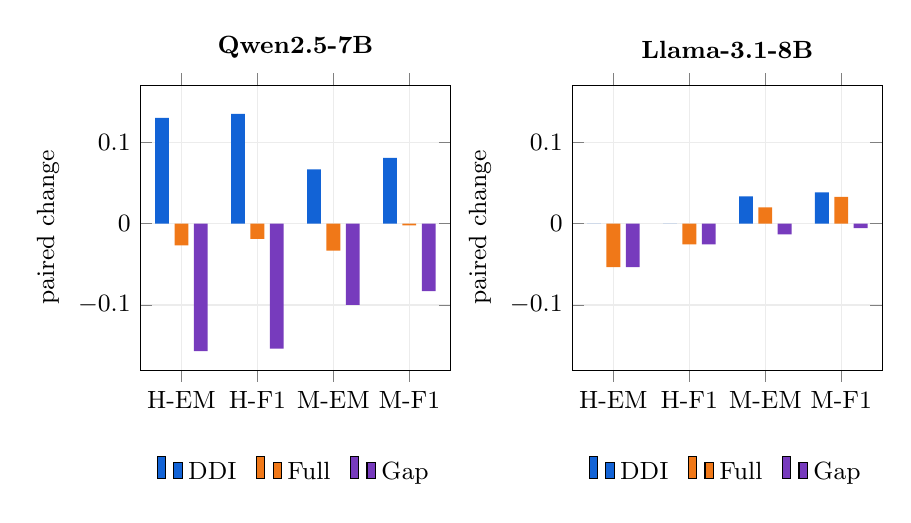
\begin{tikzpicture}
\begin{groupplot}[group style={group size=2 by 1,horizontal sep=1.55cm},width=.455\linewidth,height=5.2cm,grid=major,grid style={gray!15},tick label style={font=\small},label style={font=\small},title style={font=\small\bfseries},legend style={font=\small,draw=none,at={(.5,-.28)},anchor=north,legend columns=2,/tikz/every even column/.append style={column sep=5pt}}]
\nextgroupplot[title={Qwen2.5-7B},ylabel={paired change},xtick={0,1,2,3},xticklabels={H-EM,H-F1,M-EM,M-F1},ymin=-.18,ymax=.17,ybar,bar width=5pt,enlarge x limits=.18,legend columns=3]
\addplot[fill=ddiBlue,draw=none] coordinates {(0,0.130000) (1,0.134740) (2,0.066667) (3,0.080792)};
\addplot[fill=ddiGold,draw=none] coordinates {(0,-0.026667) (1,-0.018846) (2,-0.033333) (3,-0.002098)};
\addplot[fill=ddiPurple,draw=none] coordinates {(0,-0.156667) (1,-0.153586) (2,-0.100000) (3,-0.082890)};
\legend{DDI,Full,Gap}
\nextgroupplot[title={Llama-3.1-8B},ylabel={paired change},xtick={0,1,2,3},xticklabels={H-EM,H-F1,M-EM,M-F1},ymin=-.18,ymax=.17,ybar,bar width=5pt,enlarge x limits=.18,legend columns=3]
\addplot[fill=ddiBlue,draw=none] coordinates {(0,0.000000) (1,0.000012) (2,0.033333) (3,0.038378)};
\addplot[fill=ddiGold,draw=none] coordinates {(0,-0.053333) (1,-0.025424) (2,0.020000) (3,0.032865)};
\addplot[fill=ddiPurple,draw=none] coordinates {(0,-0.053333) (1,-0.025436) (2,-0.013333) (3,-0.005513)};
\legend{DDI,Full,Gap}
\end{groupplot}
\end{tikzpicture}

\caption{Equal-seed means of paired training changes. H/M denote Hotpot/MuSiQue.
Qwen's positive DDI changes coexist with negative full-path changes. Llama's
Hotpot gap narrowing largely reflects full-path degradation. Bars are point
estimates, not an architecture-equivalence or parity test.}
\end{figure}

Neither architecture reaches natural-QA parity under the retained rules. The
only valid original architecture contrast is MuSiQue F1: Llama minus Qwen
$C=+0.028$, equal-seed interval $[-0.085,+0.179]$. This does not establish a
practical architecture difference or equivalence. Blind-control movement
invalidates Llama Hotpot; insufficient headroom/preservation invalidates other
specified cells. Small remaining gaps alone cannot override those gates.

V54's post-hoc sensitivity jointly resamples common record IDs across the six
arms and both architectures within each seed (10,000 draws, RNG seed 54).
It does not resample a population of training seeds. Conditional intervals for
Qwen DDI F1 change are $[+.095,+.176]$ on Hotpot and $[+.042,+.120]$ on MuSiQue.
They clarify the observed training changes but do not replace the original
decision procedure. Full results and inputs are in
\path{experiments/transfer_v54_posthoc_sensitivity.json} and
\path{experiments/transfer_v54_inputs.json}; see \path{VIBEQUEUE-54-REPORT.md}.

\newpage
\section{Cache Anatomy and Provenance}
\label{app:cache}

\paragraph{Request-level derivation.}
The postprocessor reads the hash-pinned V53 compact summary, 540 timing rows
and 192 validation rows. It requires all $(\mathrm{seed},\mathrm{request},
\mathrm{mode})$ keys, exact five-by-500 document geometry, query length 32,
16 generated IDs and 15 decode forwards. Measured requests are indices 10--59;
the corresponding validation case is \texttt{stream\_k}, without renumbering.
Cached/fresh generated IDs must match those retained in validation. The
renderer recomputes each QPS as $50/\sum t_i$ and checks the compact summary.
Grouping uses hits in the \emph{timing} cache, not the separate validation cache.

\begin{table}[H]
\centering\small% Generated by paper/render.py; aggregates: paper/evidence.json.
% Sources: VIBEQUEUE-53-REPORT.md sha256=7cd9223e128c5d82b61e59575035fe4bb54c9f48c5da721723fd5d214d85195e; results/cache_v53_local_20260907/summary.json sha256=28ae886d9dae851ed090b7ebb0744b33926060d9499c3f16a01221810a0e2189; results/cache_v53_local_20260907/timing.jsonl sha256=055cf47312269ca147c6d4517d26b82aabc910b11fd6ca07f5eba5e3f54153a8; results/cache_v53_local_20260907/validation.jsonl sha256=8597c0b5394b4b17248065ad1ebc386a0a2d864f089f8e65d51d5e293f7b8d4a
\resizebox{\linewidth}{!}{%
\begin{tabular}{rrrrrrr}
\toprule
Hits & $n$ & Seed counts (0/1/2) & Equal IDs & Cache ms & Fresh ms & Paired ratio \\
\midrule
3 & 4 & 1/1/2 & 4/4 & 729.8 & 627.1 & 0.865 \\
4 & 33 & 11/12/10 & 28/33 & 606.5 & 625.4 & 1.034 \\
5 & 113 & 38/37/38 & 99/113 & 498.3 & 626.8 & 1.259 \\
\bottomrule
\end{tabular}}

\caption{Post-hoc measured hit bins. Cache/fresh milliseconds are medians on
matched requests; the last column is the median of within-request fresh/cache
latency ratios, not the ratio of medians. Equal IDs counts exact 16-token
sequence agreement. Small bins and unequal seed composition preclude a causal
hit-rate effect. No request-level confidence intervals are asserted.}
\end{table}

\paragraph{Behavioral anatomy.}
Each seed validates cold, warm, permuted and partial-reuse cases plus all 60
stream requests. Greedy failures are 0, 6 and 19 of 64 comparisons by seed;
measured-stream failures are 0, 4 and 15 of 50. The additional failures comprise
five warmup requests and one explicit permutation. Every numerical comparison
fails the unchanged $10^{-4}$ absolute/relative gate. All 384 natural-generation
outputs reach the 16-token cap; no early EOS was observed in this exact-ID stream.
Natural checks reuse already populated validation entries and are not cold
latency measurements. Teacher-forced comparisons follow fresh DDI tokens to
keep same-prefix logit errors meaningful after greedy trajectories diverge.

For example, seed 1 \texttt{stream\_7} differs at its first token: fresh chooses
220, cache 198. The fresh top-two margin is .125, the cache margin zero, and
maximum first-step logit error .21875. This is consistent with argmax changes
near a tie; it does not identify a kernel-level root cause or prove an adequate
precision fix. A passing tiny fp32 CPU test cannot establish full-model bf16
equivalence. These examples are diagnostic, not a QA correctness judgment.

\paragraph{Three generations must remain separate.}
The pre-V51 1.72$\times$ claim is withdrawn because the benchmark populated
but did not consume real KVs. V51's real-cache 1.219$\times$ claim is also
withdrawn: random IDs were decoded and retokenized, changing nominal lengths,
and full versus DDI decode work was not contractually equal. V53 is a new
exact-ID diagnostic on a different torch runtime, not an identical replication.
Its seed-wise rates must not be pooled with either older campaign.

\paragraph{Source identity and scope.}
The V53 manifest hashes checkpoint/tokenizer contents and preserves executing
sources. Base SHA is \texttt{16dd67d7e53a8168cf6580e6d0197c219e6ba198}; the
diagnostic script was untracked at launch, despite an empty tracked diff.
The manifest says \texttt{clean\_revision=false}, and both manifest and summary
say \texttt{admissible\_paper\_evidence=false}. The report remains unchanged:
\path{VIBEQUEUE-53-REPORT.md}. Exact inputs, logits, source snapshots and audit
live under \path{results/cache_v53_local_20260907/}. This paper additionally pins
the compact summary/timing/validation byte sizes and full SHA-256 values in
\path{paper/evidence.json}; hashes make postprocessing reproducible, not the
execution clean or correctness-preserving.

\paragraph{Where the optimized warm-path win came from (V69).}
The audited all-hit reuse acceleration of the main text (221.24\,ms before the
V65 optimizations, 62.30\,ms after, 3.55$\times$) is attributed by a
derivation over pinned artifacts, not by a new run: the pre/post totals trace
to the confirmation-frozen V60/V65 runs (V64-adjudicated) and the phase leaves
are uniformly rescaled from the V65 overhead profile (factor 0.945248).
Store-time validation markers remove 85.61\,ms (53.9\% of the reduction) and
the 2\,GiB LRU resident tier removes the synchronous per-document disk load of
59.14\,ms (37.2\%); the remaining 14.20\,ms (8.9\%) is a bounded envelope
within the pre-optimization cache\_assemble budget --- inferred, not directly
measured --- and the unattributed wall remainder is 3.48\,ms (1.6\% of the
pre-total, within the declared 5\% tolerance). Development-role evidence; it
supports no confirmation-quality claim.

\begin{table}[H]
\centering\small% Generated by paper/render.py from paper/evidence.json.
% Sources: results/v69_attribution_20260910T162613Z/attribution.json sha256=90f34eec2d9b24426a0af79ba757bedad178b8cb1abecf503cb0a87aea2188d1.
\begin{tabular}{llrr}
\toprule
Optimization (V65) & Pre-optimization phase removed/reduced & ms removed & \% of reduction \\
\midrule
OPT-1 store-time validation markers & validate\_entry (per-request geometry+isfinite scan) & 85.61 & 53.9 \\
OPT-2 2 GiB LRU resident tier & disk\_load (synchronous per-doc torch.load) & 59.14 & 37.2 \\
OPT-3 single staged pinned H2D copy per layer (bounded envelope) & cache\_assemble (per-entry .to(device) + cat) & 14.20 & 8.9 \\
\midrule
Total removed & & 158.94 & 100.0 \\
\midrule
\multicolumn{4}{l}{Pre-optimization all-hit reuse 221.24 ms $\to$ post-optimization 62.30 ms (3.55$\times$).} \\
\multicolumn{4}{l}{OPT-3 is a bounded envelope, not a direct measurement: it fits within the 23.04 ms pre-optimization} \\
\multicolumn{4}{l}{cache\_assemble budget; the implied post-optimization assemble of 8.84 ms is inferred, not measured.} \\
\multicolumn{4}{l}{Unattributed wall remainder 3.48 ms (1.6\% of the pre-total, within the declared 5\% tolerance).} \\
\bottomrule
\end{tabular}

\caption{Attribution of the 221.2\,ms $\to$ 62.3\,ms all-hit reuse reduction
(V69 derivation over pinned V60/V65 artifacts). OPT-1 and OPT-2 are measured
pre-optimization phases removed by the V65 changes; OPT-3 is a bounded
envelope, not a direct measurement. Development-role evidence; no
confirmation-quality claim.}
\label{tab:v69attribution}
\end{table}

\newpage
\section{Artifact Ledger and Missing Joint Design}
\label{app:ledger}

Paths below are relative to the repository root. The authoritative full hashes
and byte sizes are in \path{paper/evidence.json}. No report was modified to
retroactively admit a result. \path{paper/generated/analysis.json} contains the
new request-bin statistics, seed QPS and retained failure totals.

\begin{small}
\begin{tabular}{@{}p{2.2cm}p{8cm}p{5.2cm}@{}}
\toprule
Evidence & Exact artifacts & Row selection and unit \\
\midrule
Q1 / T2 & \path{results/runs.jsonl}; \path{results/sprint_a_strict_base.jsonl} &
\texttt{phase2\_train\_free}, Qwen-7B; tags \texttt{88162acd}/\texttt{fee7d916}; 100 IDs per arm. \\[6pt]
Q2 / T5 & \path{results/phase3_n2.jsonl}, \path{results/phase3_n5.jsonl}, \path{results/phase3_n10.jsonl} &
Hotpot full/QF, seed 0, tag \texttt{3a59828b}; match final ID suffix. \\[6pt]
P1 / T3 & \path{results/runs.jsonl} &
\texttt{phase3\_timing}, Qwen-7B, \texttt{L=512:Q=64}, SDPA, tag \texttt{88162acd}. \\[6pt]
Q3 / V54 & \path{experiments/transfer_v54_inputs.json}; \path{experiments/transfer_v54_posthoc_sensitivity.json} &
12 prediction paths; pair dataset/seed/record ID across six arms and architectures. \\[6pt]
C1 / V53 & \path{results/cache_v53_local_20260907/summary.json}, \path{timing.jsonl}, \path{validation.jsonl} in that directory &
Timing: \texttt{warmup=false}; join seed/request to validation \texttt{stream\_k}. \\
\bottomrule
\end{tabular}
\end{small}

\paragraph{Checkpoint identity cannot be inferred from the display label.}
Q2's raw run IDs name the base model, but
\path{scripts/phase3_doc_sweep2.sh} and
\path{logs/phase3_doc_sweep2.log} identify the checkpoint
\path{results/checkpoints/Qwen__Qwen2.5-7B-Instruct__ddi_qf__8L}.
File-specific Q2 config hashes are \texttt{94b5cfd00bbc44e0},
\texttt{59a0f85d992e8ca4}, and \texttt{b5f6c833f633be8e}. Do not aggregate all
base-labeled rows in the shared historical store. Q3 instead records
\texttt{checkpoint\_revision} and separate base/tuned identities in predictions.
Its exact per-seed manifests are under \path{results/transfer_heldout/}.

\paragraph{Schemas and missing fields.}
Legacy scalar JSONL has \texttt{run\_id, metric, value, provenance}; quality
record IDs are the run-ID suffix. Modern predictions have a separate
\texttt{record\_id}, decoded prediction, possible answers, a four-metric object,
and provenance. Neither QA schema stores per-record prefill times, document
token lengths or cache hit states. Timing repeats are JSON strings inside the
scalar \texttt{value}. V53 has request-level geometry, IDs, hits and latency,
but no gold QA answers. These schema differences explain the missing cells in
Figure~\ref{fig:coverage}; matching only the model and mask is not enough.

\paragraph{Historical Flex lineage.}
Figure~\ref{fig:flexhistory} parses detailed milliseconds, not rounded ratios,
from hash-pinned \path{logs/timing_flex2.log} and
\path{logs/timing_flex_model3.log}. The scripts preserved at Git revision
\texttt{2029129}, \path{scripts/timing_flex_test.py} and
\path{scripts/timing_flex_model.py}, distinguish raw Q/K/V timing from the
whole-model forward. Their document mask lacks an intra-document causal
condition. Preserved logs establish reported timings, not exact launch-source
identity or current-mask parity. The separate 3.98$\times$ archived claim is
recorded in that revision's changelog; absent its matching raw log, it remains
unplotted. The old square-matrix sparsity summaries are not reused.

\paragraph{Minimum future joint record.}
Retain an immutable request ID, exact document/query IDs, gold answers,
checkpoint/tokenizer/source hashes, mask/layout, cache namespace and pre-state,
hit identities, actual geometry, generated IDs and stopping reason. Record
natural-generation EM/F1 separately from fixed-work TTFT, end-to-end time and
decode forwards. Randomize or counterbalance execution order and preserve
per-seed pairing. Evaluate cold/warm/reordered/partial states and a real
optimized prefix-cache baseline before claiming an advantage over prefix reuse.

Reports \path{VIBEQUEUE-54-REPORT.md}, \path{VIBEQUEUE-53-REPORT.md},
\path{VIBEQUEUE-55-REPORT.md} and \path{EVIDENCE_TO_CLAIM.md} define the retained
estimands, withdrawals and failed kernel gates. A future matched campaign may
fill the coverage map; the present appendix does not count that unrun design
as an experiment or relax any original gate.


\end{document}
